\documentclass[12pt,a4paper]{article}
\usepackage[UTF8]{ctex}
\usepackage{amsmath}
\usepackage{amssymb}
\usepackage{geometry}
\usepackage{booktabs}
\usepackage{graphicx}
\usepackage{float}

\geometry{left=2.5cm,right=2.5cm,top=2.5cm,bottom=2.5cm}

\title{三相异步电机实验报告}
\author{}
\date{}

\begin{document}

\maketitle
\newpage
\tableofcontents
\newpage
\section{实验目的}

\begin{enumerate}
    \item 测量异步电动机定子绕组电阻；
    \item 测取并分析异步电动机的空载特性 $I_0$、$p_0 = f(U_0)$；
    \item 测取并分析异步电动的短路特性 $I_k$、$p_k = f(U_k)$；
    \item 通过空载和短路特性计算的异步电动机的 T 形等值电路；
    \item 测取异步电动机的机械特性 $n = f(T_2)$；
    \item 测取并分析异步电动机的工作特性 $\eta$、$I_1$、$T_1$、$n$、$\cos\varphi = f(P_2)$；
    \item 利用 Y-$\Delta$ 起动电路完成电机降压起动；
    \item 测取异步电动机的转子回路串电阻调速和调压调速特性；
\end{enumerate}

\section{实验对象}

绕线式异步电动机，型号 M09-A。

额定参数：

\begin{itemize}
    \item 额定功率 $P_N = 100$ W
    \item 额定电压 $U_N = 220$ V (Y)
    \item 额定频率 $f_N = 50$ Hz
    \item 额定电流 $I_N = 0.55$ A
    \item 额定转速 $n_N = 1420$ rpm
\end{itemize}

\section{实验项目}
\subsection{实验台编号 10}
\subsection{环境温度15℃}
\subsection{定子绕组电阻测量}

直接使用数字万用表分别测量三相定子绕组电阻，电路图略。

数字万用表型号 \underline{FLUKE\quad 17B+\hspace{5cm}}，

测量量程 \underline{Auto\hspace{3cm}}，

$R_A = $ \underline{13.1\hspace{3cm}}$\Omega$，
$R_B = $ \underline{13.3\hspace{3cm}}$\Omega$，
$R_C = $ \underline{13.7\hspace{3cm}}$\Omega$。

\subsection{空载试验}

实验电路图如图 3-1 所示，图中所选用的设备列在表 \ref{1} 中。

确认三相调压器 AT 输出置零，机械负载调至最小，合上电源，逐渐升高电压起动电机。调节施加空载电压 $U_0$ 由 260V（$1.2U_N$）逐渐降低，直到定子电流开始回升，转差率显著增大为止。这个过程测取 8 个点，每个点要求记录空载电压 $U_{AB}$、$U_{BC}$、$U_{AC}$，空载电流 $I_A$、$I_B$、$I_C$，空载功率 $P_{\text{I}}$、$P_{\text{II}}$。这里的空载电压 $U_0$ 为三个线电压的平均值。
\begin{figure}[H]
    \centering
    
\includegraphics[width=1\textwidth]{./images/1.png}
\end{figure}
\begin{table}[h]
\centering

\caption{异步机空载（负载）实验的仪表选用}
\begin{tabular}{ccc}
\toprule
位号 & 类型 & 说明 \\
\midrule
AT & 三相交流电源 & MEL-002T 三相可调电源 \\
$U_{AB}$, $U_{BC}$, $U_{AC}$ & 交流电压表 & NEEL-001A 测量电机线电压 \\
$I_A$, $I_B$, $I_C$ & 交流电流表 & NEEL-001A 测量电机线电流 \\
$P_{\text{I}}$, $P_{\text{II}}$ & 功率表 & NEEL-001A 测取三相有功功率 \\
TG & 机械负载 & NMEL-13A 包括涡流测功机及其附属设备，含测速功能 \\
\bottomrule
\end{tabular}
\label{1}
\end{table}

\begin{table}[H]
\centering
\caption{异步电动机空载试验数据记录}
\begin{tabular}{cccccccc}
\toprule
$U_{AB}$ (V) & $U_{BC}$ (V) & $U_{AC}$ (V) & $I_A$ (A) & $I_B$ (A) & $I_C$ (A) & $P_{\text{I}}$ (W) & $P_{\text{II}}$ (W) \\
\midrule
262.4 & 260.6 & 258.7 & 0.51 & 0.49 & 0.47 & -37 & 73.6 \\
236.7 & 234.8 & 233.9 & 0.437 & 0.415 & 0.395 & -26.7 & 58.53 \\
212.5 & 210.3 & 209.6 & 0.378 & 0.364 & 0.342 & -17.3 & 47.18 \\
186.2 & 184.5 & 184.2 & 0.323 & 0.32 & 0.3 & -12 & 38.28 \\
161 & 160 & 160.5 & 0.274 & 0.277 & 0.264 & -6.84 & 31.73 \\
136 & 134.9 & 135.8 & 0.238 & 0.247 & 0.228 & -1.93 & 25.14 \\
110.3 & 109 & 110.1 & 0.21 & 0.228 & 0.209 & 1.58 & 20.2 \\
84.43 & 84.33 & 85.89 & 0.196 & 0.211 & 0.217 & 3.37 & 17.92 \\
\bottomrule
\end{tabular}
\end{table}

\subsection{短路试验}

实验电路图如图 3-2 所示，图中所选用的设备列在表 \ref{1} 中。

首先检查电动机旋转方向，使用适当的方法堵住转子。注意，防止堵转子的制动工具抛出伤人。确认三相调压器 AT 输出置零，合上电源。逐渐升高施加电压，使短路电流 $I_k$ 升至 0.66A（$1.2I_N$），再逐渐降低电压使电流降至 0.16A（$0.3I_N$）左右，这个过程测取 5 个点，每个点需要测取短路电流 $I_A$、$I_B$、$I_C$，短路电压 $U_{AB}$、$U_{BC}$、$U_{AC}$，短路功率 $P_{\text{I}}$、$P_{\text{II}}$。这里的短路电流 $I_k$ 为三个线电流的平均值。
\begin{figure}[H]
    \centering
    
\includegraphics[width=1\textwidth]{./images/2.png}
\end{figure}

\begin{table}[H]
\centering
\caption{异步电动机短路试验数据记录}
\begin{tabular}{cccccccc}
\toprule
$U_{AB}$ (V) & $U_{BC}$ (V) & $U_{AC}$ (V) & $I_A$ (A) & $I_B$ (A) & $I_C$ (A) & $P_{\text{I}}$ (W) & $P_{\text{II}}$ (W) \\
\midrule
59.42 & 60.29 & 58.73 & 0.658 & 0.664 & 0.664 & -35.8 & -2.74 \\
51.92 & 52.27 & 51.53 & 0.572 & 0.578 & 0.575 & -27 & -1.96 \\
45.27 & 45.52 & 45.04 & 0.5 & 0.504 & 0.504 & -20.9 & -1.59 \\
38.48 & 38.97 & 38.50 & 0.417 & 0.429 & 0.421 & -14.7 & -1.71 \\
31 & 31.53 & 30.51 & 0.332 & 0.345 & 0.33 & -9.47 & -1.06 \\
23.39 & 24.42 & 23.58 & 0.254 & 0.263 & 0.261 & -5.43 & -0.91 \\
14.37 & 15.28 & 14.3 & 0.151 & 0.167 & 0.167 & -2 & -0.41 \\
\bottomrule
\end{tabular}
\label{2}
\end{table}

\subsection{负载试验}

实验电路图如图 3-1 所示，图中所选用的设备列在表 \ref{1} 中。

机械负载调至最小，校零 TG 中的转矩测量传感器。确认三相调压器 AT 输出置零，合上电源，逐渐升高电压起动电机，调节电机输入线电压 $U_1$ 至 220V（$U_N$）。调节机械负载 TG，使电动机负载电流 $I_1$ 上升至 0.66A（$1.2I_N$）。然后逐级减小负载，直至空载或负载最小，同时保持输入电压始终为 220V，测取 6 个点。每个点需要记录三相线电流 $I_A$、$I_B$、$I_C$，电机输入功率 $P_{\text{I}}$、$P_{\text{II}}$，输出转矩 $T_2$ 和输出转速 $n$。

\begin{table}[H]
\centering
\caption{异步电动机负载试验数据记录}
\begin{tabular}{ccccccccc}
\toprule
$U_{n}$ (V) & $I_a$ (A) & $I_{b}$ (A) & $I_c$ (A) & $P_{\text{I}}$ (W) & $P_{\text{II}}$ (W) & $T_{2}$ (N*m) & $n$ (rpm) \\
\midrule
220&	0.673&	0.666&	0.636&	54.69&	136.1&	1.04&	1370\\
220&	0.585&	0.575&	0.533&	39.96&	113.1&	0.82&	1395\\
220&	0.505&	0.5&	0.466&	21.65&	95.22&	0.61&	1420\\
220&	0.462&	0.467&	0.437&	12.06&	85.91&	0.5&	1431\\
220&	0.44&	0.441&	0.418&	4.57&	78&	0.41&	1440\\
220&	0.39&	0.4&	0.372&	-12.5&	60.6&	0.2&	1463\\
220&	0.378&	0.393&	0.367&	-22.1&	50.61&	0&	1478\\
\bottomrule
\end{tabular}
\end{table}

\subsection{异步电机 Y-$\Delta$ 起动}

实验电路如图 3-3 所示，图中所选用的设备列在表\ref{2} 中。

断开 $K_1$，确认调压器 AT 输出置零，合上电源。调节调压器 AT 使线电压 $U$ 为 127V（$U_N/\sqrt{3}$）。$K_2$ 设置为 Y 模式，合上 $K_1$，稳定运行后，记录 Y 形时电流 I 的大小。将 $K_2$ 切换为 $\Delta$ 模式，稳定运行后，记录 $\Delta$ 形时电流 I 的大小。
\begin{figure}[H]
    \centering
    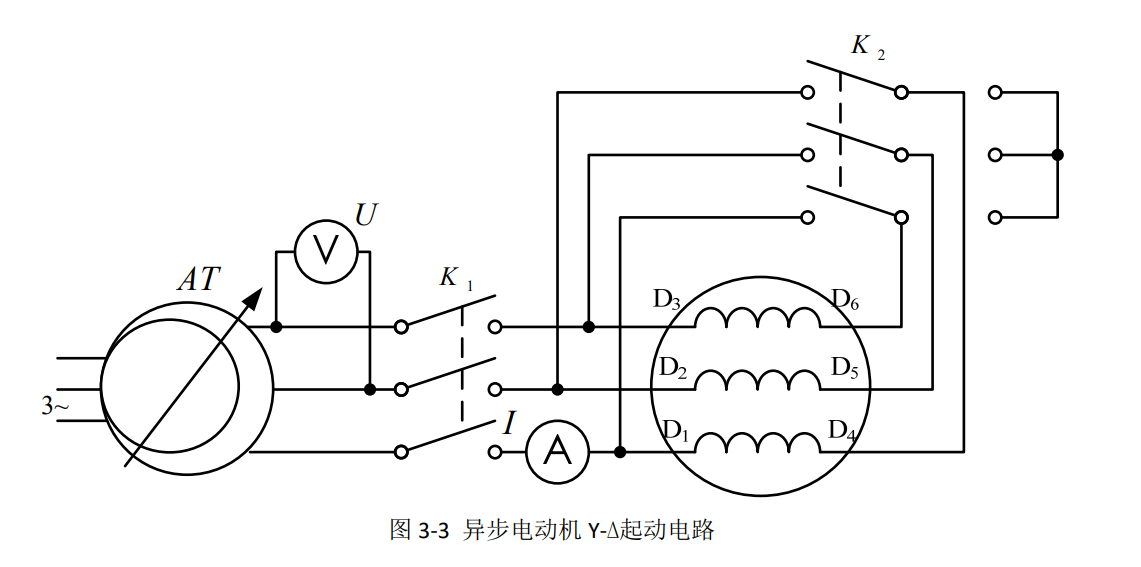
\includegraphics[width=1\textwidth]{./images/3.png}
\end{figure}
\begin{table}[h]
\centering

\caption{异步机 Y-$\Delta$ 起动实验的仪表选用}
\begin{tabular}{ccc}
\toprule
位号 & 类型 & 说明 \\
\midrule
AT & 三相交流电源 & MEL-002T 三相可调电源 \\
$U$ & 交流电压表 & NEEL-001A \\
$I$ & 交流电流表 & NEEL-001A \\
$K_1$, $K_2$ & 开关 & NMEL-05B 三刀双掷开关 \\
\bottomrule
\end{tabular}
\label{2}
\end{table}

\vspace{1cm}

Y 形时电流 $I_Y =$ \underline{ 0.215\hspace{3cm}} A

$\Delta$ 形时电流 $I_\Delta = $ \underline{  0.63\hspace{3cm}} A

\subsection{异步电动机调速}

实验电路如图 3-4 所示，图中所选用的设备列在表 6 中。
\begin{figure}[H]
    \centering
    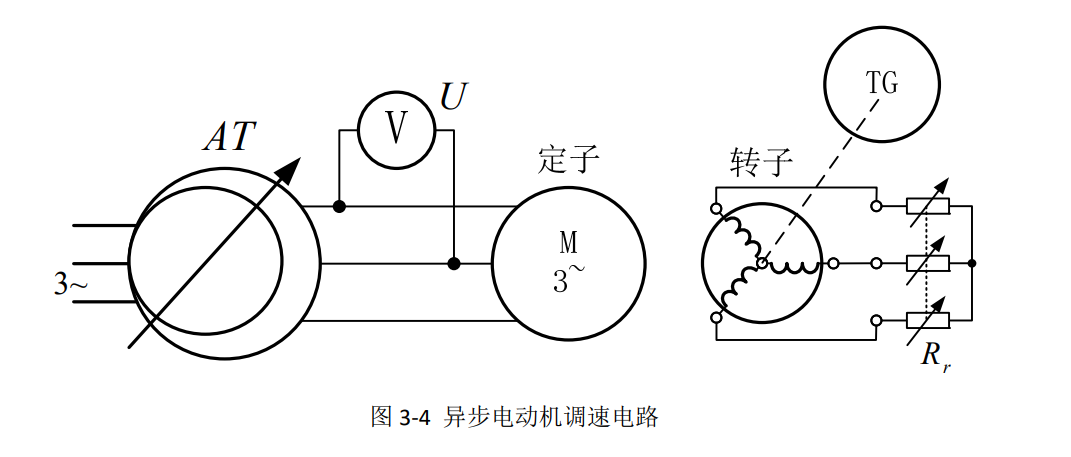
\includegraphics[width=1\textwidth]{./images/4.png}
\end{figure}
\begin{table}[h]
\centering
\caption{异步机调速实验的仪表选用}
\begin{tabular}{ccc}
\toprule
位号 & 类型 & 说明 \\
\midrule
AT & 三相交流电源 & MEL-002T 三相可调电源 \\
$U$ & 交流电压表 & NEEL-001A \\
$R_r$ & 绕线电机起动电阻 & NMEL-03/4 \\
TG & 机械负载 & NMEL-13A 包括涡流测功机及其附属设备，含测速功能 \\
\bottomrule
\end{tabular}
\end{table}

机械负载调至最小，校零 TG 中的转矩测量传感器。转子电阻 $R_r$ 置为 0，合上电源。调节调压器 AT 起动电机，保持机械负载最小，调节线电压 $U$ 由 220V（$U_N$）逐渐降低到 88V（$0.4U_N$），这个过程测取 5 个点，每个点记录线电压 $U$ 和转速 $n$。

改变机械负载为 0.2Nm，按上面的方法重复测试。

\begin{table}[h]
\centering
\caption{异步电动机调压调速数据记录}
\begin{tabular}{cccc}
\toprule
\multicolumn{2}{c}{$T_2 = 0$ Nm, $R_r = 0$} & \multicolumn{2}{c}{$T_2 = 0.2$ Nm, $R_r = 0$} \\
\cmidrule(lr){1-2} \cmidrule(lr){3-4}
$U$ (V) & $n$ (rpm) & $U$ (V) & $n$ (rpm) \\
\midrule
220 & 1479 & 219.3 & 1464 \\
197.7 & 1471 & 197.1 & 1453 \\
176 & 1467 & 176 & 1449 \\
153.9 & 1456 & 154 & 1437 \\
131.3 & 1447 & 131.7 & 1414 \\
110.6 & 1429 & 109.5 & 1374 \\
88.33 & 1398 & 88.5 & 1287 \\
\bottomrule
\end{tabular}
\end{table}

调节线电压 $U$ 为额定值 220V（$U_N$），调节机械负载最小，逐级改变转子电阻 $R_r$，测取每个转子电阻对应的电机转速。

改变机械负载为 0.2Nm，按上面的方法重复测试。

\begin{table}[h]
\centering
\caption{异步电动机转子回路串电阻调速数据记录}
\begin{tabular}{ccccc}
\toprule
\multicolumn{5}{c}{$T_2 = 0$ Nm, $U = U_N = 220$ V} \\
\midrule
$R_r$ ($\Omega$) & 0 & 2 & 5 & 15 \\
$n$ (rpm) & 1477&	1472	&1463&	1445	\\
\midrule
\multicolumn{5}{c}{$T_2 = 0.2$ Nm, $U = U_N = 220$ V} \\
\midrule
$R_r$ ($\Omega$) & 0 & 2 & 5 & 15 \\
$n$ (rpm) &1466&	1459&	1453&	1437\\
\bottomrule
\end{tabular}
\end{table}
\section{数据处理与分析}

\subsection{定子绕组电阻}

测量结果：
\begin{equation*}
R_{a} = 13.1\Omega \quad R_{b} = 13.7\Omega \quad R_{c} = 13.3\Omega
\end{equation*}

三相平均电阻：
\begin{equation*}
R_{1} = \frac{R_{A} + R_{B} + R_{C}}{3} = 13.367\Omega
\end{equation*}

从测量结果可以看出，三相定子绕组电阻数值接近，最大偏差为
\begin{equation*}
\frac{13.7 - 13.1}{13.37} \approx 4.5\%
\end{equation*}

说明电机三相绕组对称性较好,绕组不存在明显匝间短路或接线异常，为后续空载实验结果的可靠性提供了基础条件。

\subsection{空载实验数据处理与分析}

\subsubsection{空载实验数据}

\begin{table}[H]
\centering
\small
\begin{tabular}{crrrrrrrr|rrr}
\toprule
序号 & $U_{ab}$(V) & $U_{bc}$(V) & $U_{ac}$(V) & $I_{a}$(A) & $I_{b}$(A) & $I_{c}$(A) & $P_{\text{I}}$(W) & $P_{\text{II}}$(W) & $U_{0}$(V) & $I_{0}$(A) & $P$(W) \\
\midrule
1 & 262.4 & 260.6 & 258.7 & 0.51 & 0.49 & 0.47 & -37 & 73.6 & 260.57 & 0.49 & 36.6 \\
2 & 236.7 & 234.8 & 233.9 & 0.437 & 0.415 & 0.395 & -26.7 & 58.53 & 235.13 & 0.416 & 31.83 \\
3 & 212.5 & 210.3 & 209.6 & 0.378 & 0.364 & 0.342 & -17.3 & 47.18 & 210.8 & 0.361 & 29.88 \\
4 & 186.2 & 184.5 & 184.2 & 0.323 & 0.32 & 0.3 & -12 & 38.28 & 184.97 & 0.314 & 26.28 \\
5 & 161 & 160 & 160.5 & 0.274 & 0.277 & 0.264 & -6.84 & 31.73 & 160.5 & 0.272 & 24.89 \\
6 & 136 & 134.9 & 135.8 & 0.238 & 0.247 & 0.228 & -1.93 & 25.14 & 135.57 & 0.238 & 23.21 \\
7 & 110.3 & 109 & 110.1 & 0.21 & 0.228 & 0.209 & 1.58 & 20.2 & 109.8 & 0.216 & 21.78 \\
8 & 84.43 & 84.33 & 85.89 & 0.196 & 0.211 & 0.217 & 3.37 & 17.92 & 84.88 & 0.208 & 21.29 \\
9 & 70.8 & 70.2 & 71.54 & 0.215 & 0.224 & 0.225 & 5.38 & 15.68 & 70.85 & 0.221 & 21.06 \\
\bottomrule
\end{tabular}
\end{table}

其中：
\begin{equation*}
U_{0} = \frac{U_{ab} + U_{bc} + U_{ca}}{3}, \quad I_{0} = \frac{I_{a} + I_{b} + I_{c}}{3}, \quad P = |P_1 + P_2|
\end{equation*}

\subsubsection{空载电压与空载电流特性分析}

\textbf{空载电流$I_0$随电压$U_0$的变化规律：}
\begin{figure}[H]
    \caption{空载电流与空载电压特性}
    \centering
    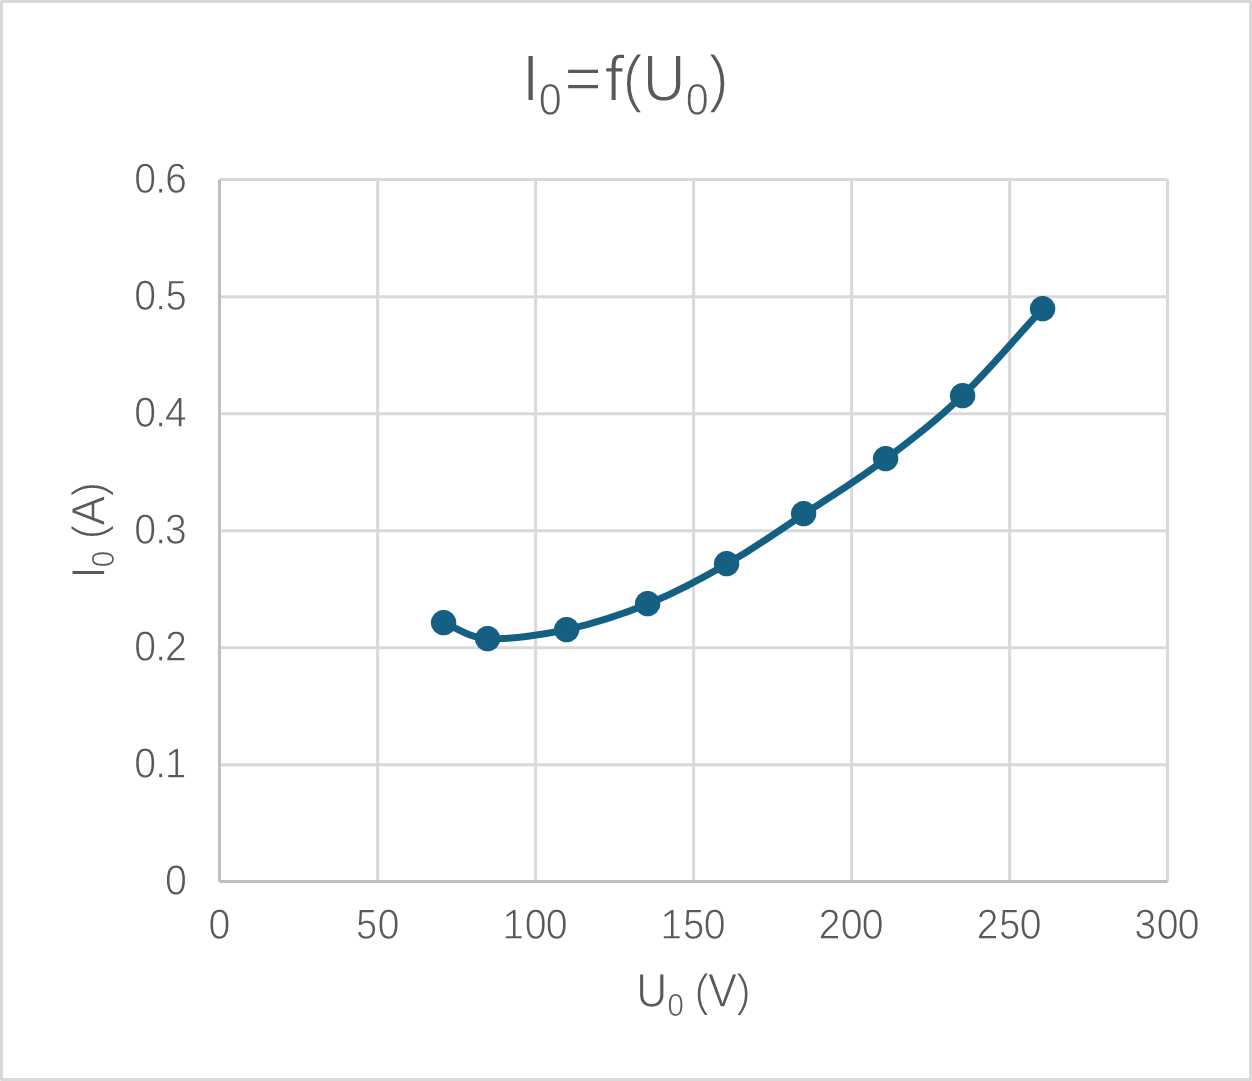
\includegraphics[width=0.7\textwidth]{./images/图片1.png}
    \label{figure:1}
\end{figure}

当$U_0$从260 V降至约135 V：$I_0$基本随电压线性减小。

当$U_0 < 100$ V：$I_0$下降趋势变缓，甚至略有回升。

由表中数据可知，空载电流$I_0$随着空载电压$U_0$的降低整体呈下降趋势。在较高电压区间(约260 V至135 V)，$I_0$与$U_0$近似呈线性关系，表明此时电机处于正常磁化区。当电压进一步降低至100 V以下时，空载电流下降趋势明显减缓，部分测点甚至出现轻微回升。这主要是由于低电压下励磁不足，电机转速下降，转差率增大，转子电流分量上升所致。该变化趋势符合异步电机空载运行的理论特性。

\subsubsection{空载功率特性分析}

\textbf{空载功率的组成：}
\begin{itemize}
\item 铁损(磁滞损耗 + 涡流损耗)
\item 机械损耗(摩擦)
\item 少量定子铜损
\end{itemize}

\textbf{空载功率随电压变化的规律：}
\begin{figure}[H]
    \centering
    \caption{空载功率与电压特性}
    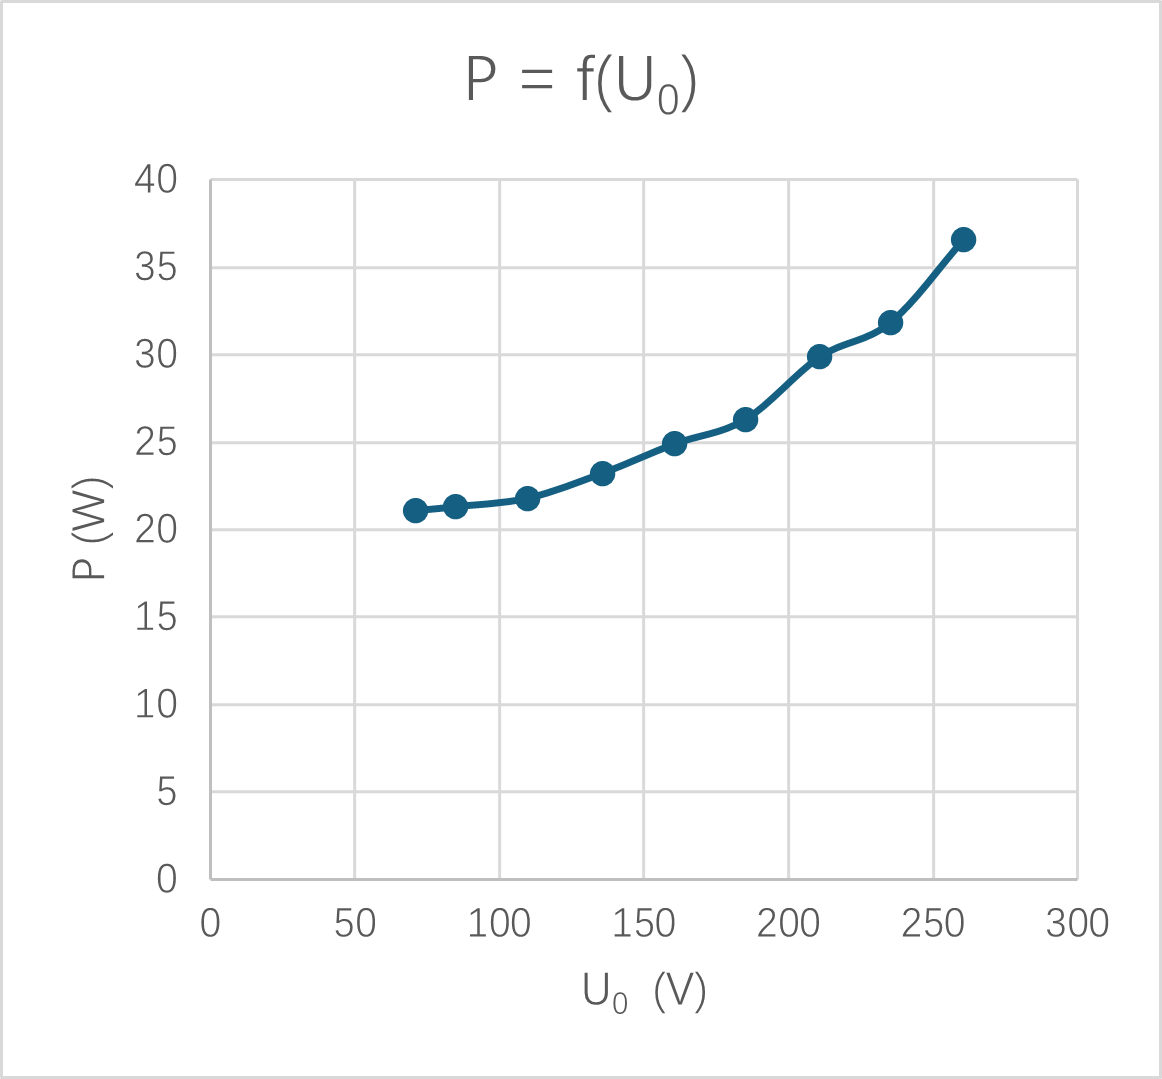
\includegraphics[width=0.8\textwidth]{./images/图片2.png}

\end{figure}
高电压区：随$U_0$明显变化

低电压区：变化趋缓，接近稳定

从实验结果可以看出，空载功率$P_0$在较高电压范围内随电压降低而明显减小，表明该区间内铁损占空载损耗的主要部分。由于铁损与磁通密切相关，而磁通又近似与电压成正比，因此功率变化较为显著。

当空载电压降低至约100 V以下时，空载功率变化趋于平缓，逐渐接近一个稳定值。这说明在低电压区间内，铁损显著减小，此时空载功率主要由机械损耗和少量铜损构成，其大小与电压关系不大。该现象与异步电机空载损耗理论分析结果一致。

在实验过程中，采用两瓦特计法测量三相功率。当功率因数较低时，其中一个瓦特计可能出现负读数。这是由于电压与电流相位差较大，导致瓦特计指针反向偏转所致。因此实验中采用$P = |P_1 + P_2|$作为三相输入功率的计算方式，该处理方法符合两瓦特计法的理论要求。

\textbf{空载实验总结：}

综上所述，通过对三相异步电机空载实验数据的分析可以得出：空载电流随电压整体呈下降趋势，空载功率在高电压区主要受铁损影响，在低电压区主要由机械损耗构成。实验结果整体符合异步电机空载运行的理论特性，说明实验过程及数据具有较好的可靠性。

\subsection{短路实验数据处理与分析}

\subsubsection{短路实验数据}

\begin{table}[H]
\centering
\small
\begin{tabular}{crrrrrrrr|rrr}
\toprule
序号 & $U_{ab}$(V) & $U_{bc}$(V) & $U_{ac}$(V) & $I_{a}$(A) & $I_{b}$(A) & $I_{c}$(A) & $P_{\text{I}}$(W) & $P_{\text{II}}$(W) & $U_{k}$(V) & $I_{k}$(A) & $P$(W) \\
\midrule
1 & 59.42 & 60.29 & 58.73 & 0.658 & 0.664 & 0.664 & -35.8 & -2.74 & 59.48 & 0.662 & 38.54 \\
2 & 51.92 & 52.27 & 51.53 & 0.572 & 0.578 & 0.575 & -27 & -1.96 & 51.91 & 0.575 & 28.96 \\
3 & 45.27 & 45.52 & 45.04 & 0.5 & 0.504 & 0.504 & -20.9 & -1.59 & 45.28 & 0.503 & 22.49 \\
4 & 38.48 & 38.97 & 38.50 & 0.417 & 0.429 & 0.421 & -14.7 & -1.71 & 38.73 & 0.422 & 16.41 \\
5 & 31 & 31.53 & 30.51 & 0.332 & 0.345 & 0.33 & -9.47 & -1.06 & 31.01 & 0.336 & 10.53 \\
6 & 23.39 & 24.42 & 23.58 & 0.254 & 0.263 & 0.261 & -5.43 & -0.91 & 23.80 & 0.259 & 6.34 \\
7 & 14.37 & 15.28 & 14.3 & 0.151 & 0.167 & 0.167 & -2 & -0.41 & 14.65 & 0.162 & 2.41 \\
\bottomrule
\end{tabular}
\end{table}

短路实验中，通过调压器逐步升高定子端电压，使电机在转子堵转(或近似堵转)状态下运行。此时电机转速接近于零，转差率$s \approx 1$，输入功率主要消耗于定、转子铜损，铁损与机械损耗可忽略不计。

实验中采用两瓦特计法测量三相输入功率，并按$P = |P_1 + P_2|$计算三相总功率。

根据实验数据计算得到三相平均短路电压与电流：
\begin{equation*}
U_{k} = \frac{U_{ab} + U_{bc} + U_{ca}}{3}, \quad I_{k} = \frac{I_{a} + I_{b} + I_{c}}{3}
\end{equation*}

从数据可以看出，在各测量点处，三相电压与三相电流数值接近，最大偏差均较小，表明电机三相绕组及实验接线具有良好的对称性，实验数据具有较好的可靠性。

\subsubsection{短路电流-电压特性分析}
\begin{figure}[H]
    \caption{短路电流与短路电压特性}
    \centering
    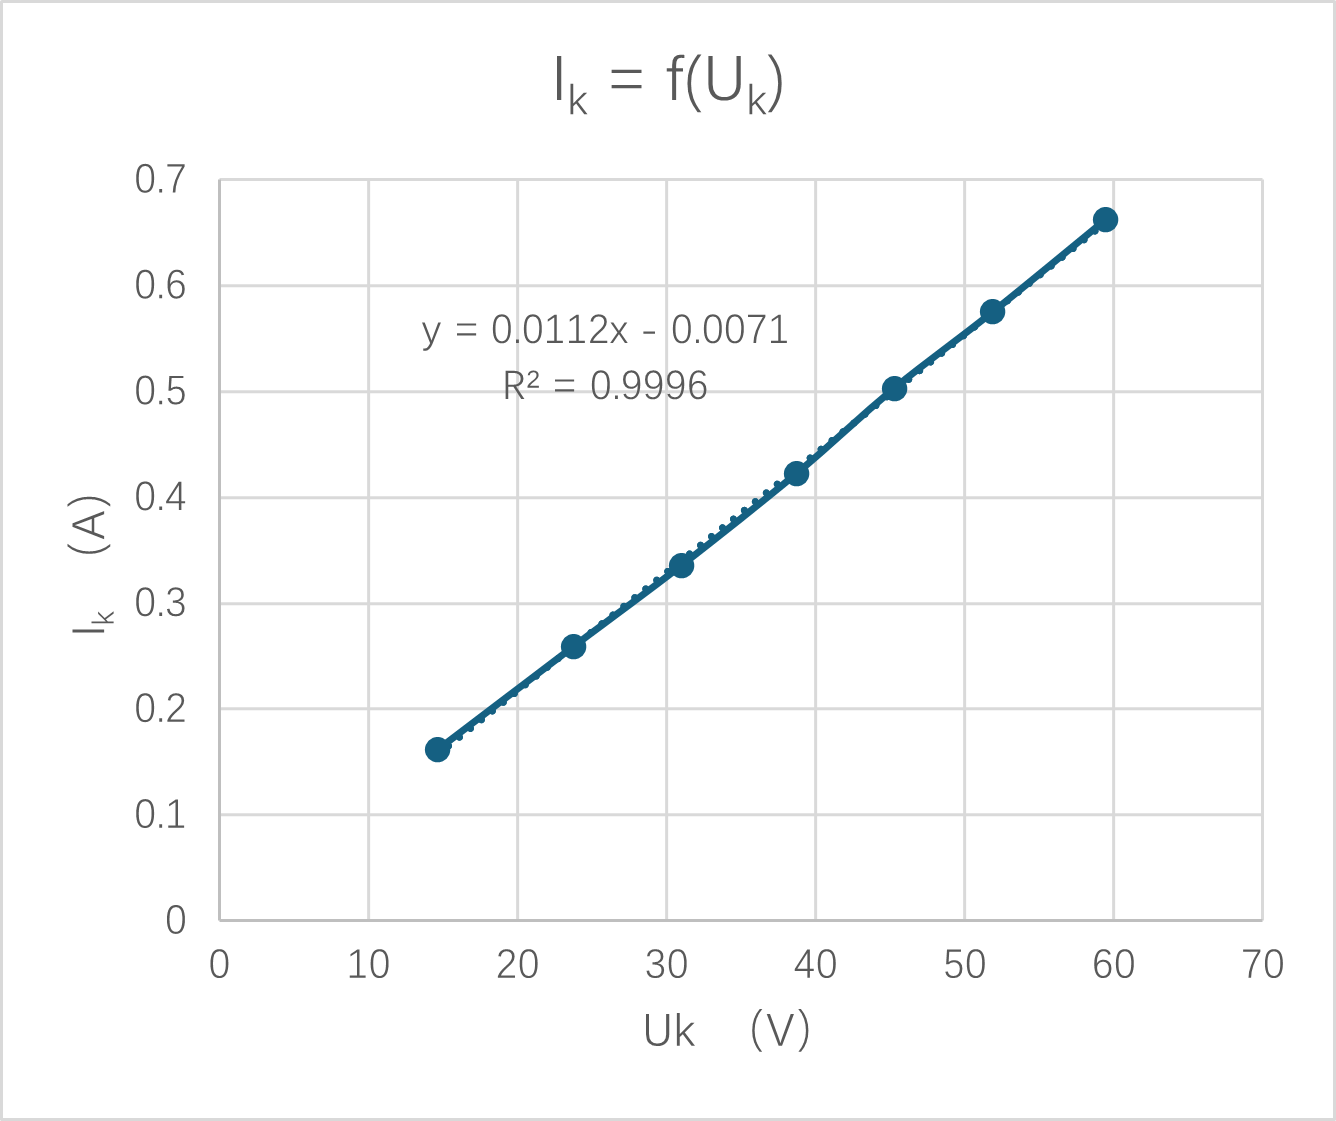
\includegraphics[width=0.8 \textwidth]{./images/图片3.png}
\end{figure}
由实验数据可知，短路电流$I_k$随短路电压$U_k$的变化关系如下：

当$U_k$从约15 V提高至60 V时，$I_k$由0.16 A近似线性增加至0.66 A。

从短路实验结果可以看出，短路电流$I_k$与短路电压$U_k$基本呈线性关系。这表明在短路实验过程中，电机磁路未进入饱和区，等效阻抗近似保持不变。由于短路实验时施加的电压较低，定子铁芯磁通较小，铁损可以忽略，因此电机等效电路中主要由定子电阻和漏抗决定电流大小，该实验结果与异步电机短路特性理论相一致。

\subsubsection{短路功率特性分析}
\begin{figure}[H]
    \caption{短路功率与短路电压特性}
    \centering
    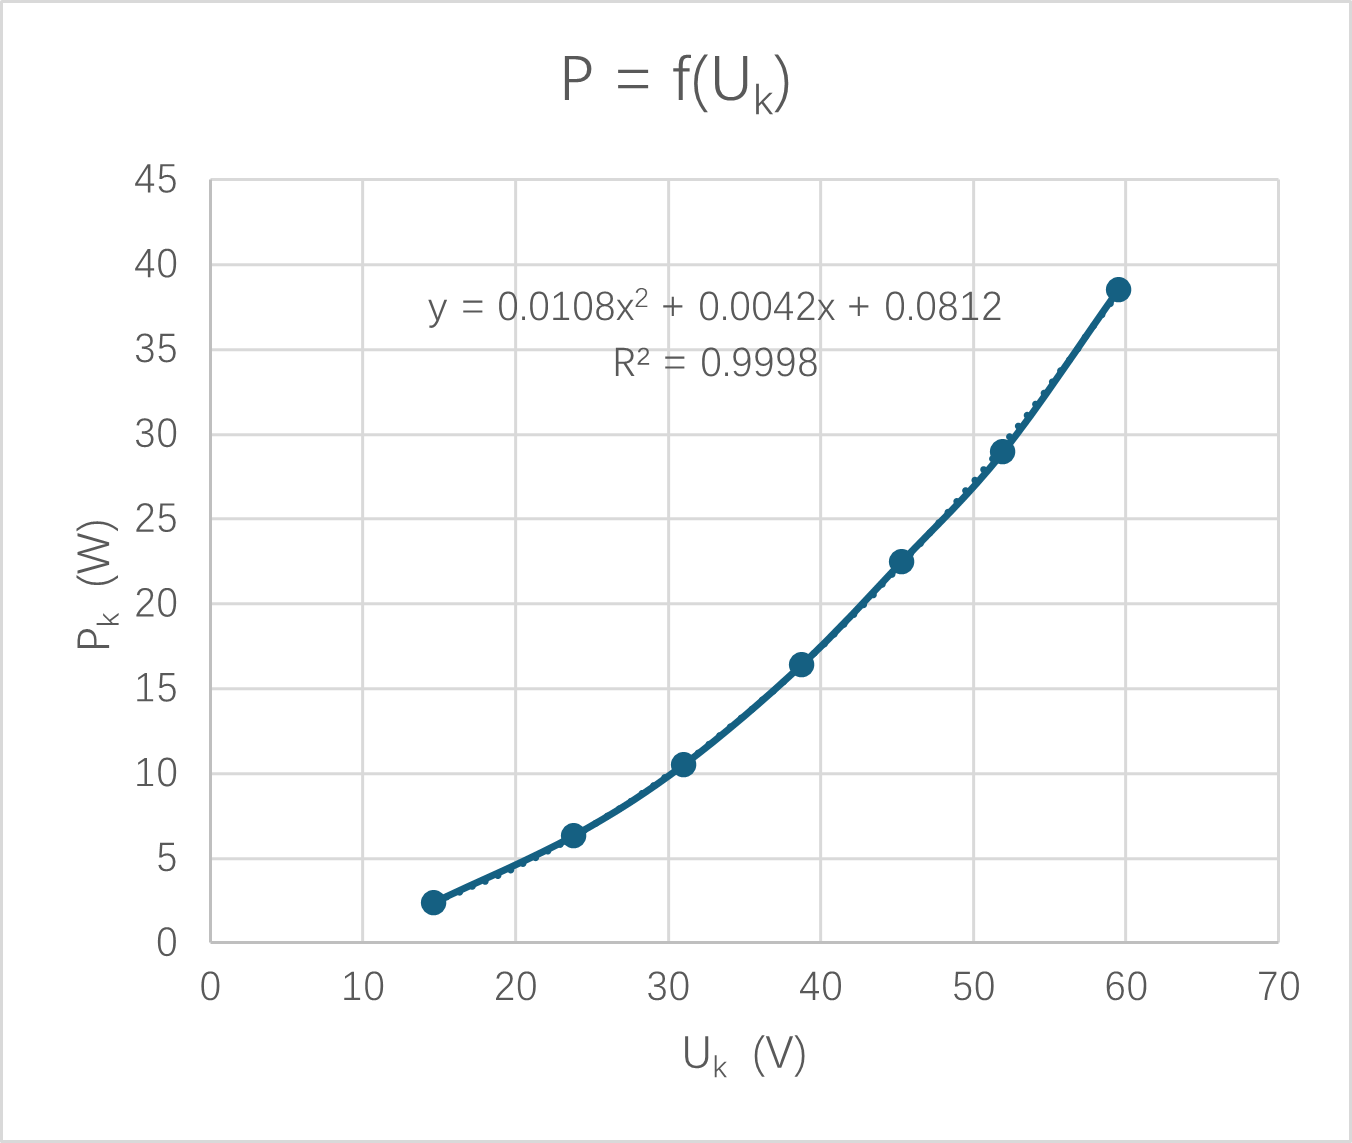
\includegraphics[width=0.8\textwidth]{./images/图片4.png}
\end{figure}
实验测得的短路功率$P_k$随短路电流变化情况如下：

随$U_k$与$I_k$的增大，短路功率明显上升，功率增长趋势近似与电流平方成正比。

由实验数据可知，短路功率$P_k$随短路电流增大而显著增加。由于短路实验时电机转速接近零，输入功率主要转化为定、转子铜损，而铜损与电流平方成正比，因此短路功率随电流上升较为迅速。实验结果表明，在短路状态下，电机功率损耗主要由绕组电阻决定，该结论为后续等值电路参数中等效电阻的计算提供了实验依据。

\textbf{短路实验结果总结：}

综上所述，通过对三相异步电机短路实验数据的分析可以得出：短路电流与短路电压之间呈近似线性关系，短路功率主要由定、转子铜损构成，与电流平方成正比，铁损与机械损耗可以忽略。实验结果整体符合异步电机短路运行的理论特性，实验数据具有较好的可靠性，可用于后续电机等值电路参数的计算。

\subsection{T型等效电路}

\subsubsection{等值电路参数计算的总体思路}

在三相异步电机实验中：
\begin{itemize}
\item 空载实验 → 求励磁支路参数
\item 短路实验 → 求串联支路参数
\end{itemize}

在实验分析中，作如下工程近似假设：
\begin{itemize}
\item 三相对称运行
\item 定、转漏抗近似相等：$X_1 \approx X_2'$
\item 短路时铁损与机械损耗可忽略
\end{itemize}

\subsubsection{定子电阻$R_1$}

测得三相定子绕组电阻平均值：
\begin{equation*}
R_1 = 13.37\Omega
\end{equation*}

折算到75℃：
\begin{equation*}
R_{1(75℃)} = \frac{234.5 + 75}{234.5 + 15}R_0 = 16.6\Omega
\end{equation*}

\subsubsection{空载实验参数计算}

1. 取额定附近空载数据点，选用接近同时大于额定电压测点(磁通最接近额定)：
\begin{equation*}
U_l = 235.13\text{ V}, \quad I_0 = 0.49\text{ A}, \quad P_0 = 36.6\text{ W}
\end{equation*}

2. 相电压计算(Y接)：
\begin{equation*}
U_{0\phi} = \frac{U_0}{\sqrt{3}} = \frac{235.13}{\sqrt{3}} \approx 135.8\text{ V}
\end{equation*}

3. 定子铜损：
\begin{equation*}
P_{cu1,0} = 3I_0^2 R_1 = 3 \times (0.416)^2 \times 16.6 \approx 8.655\text{ W}
\end{equation*}

4. 空载损耗(铁损 + 机械损耗)：
\begin{equation*}
P_{fe + fw} = P_0 - P_{cu1,0} = 31.83 - 8.655 = 23.175\text{ W}
\end{equation*}

5. 励磁电阻$R_m$：
\begin{equation*}
R_m = \frac{P_{fe + fw}}{3I_0^2} = 44.64\Omega
\end{equation*}

6. 励磁电流：
\begin{equation*}
I_m = \sqrt{I_0^2 - I_{fe}^2} \approx I_0 = 0.41\text{ A}
\end{equation*}

7. 空载阻抗：
\begin{equation*}
Z_0 = \frac{U_{0\phi}}{I_0} = \frac{135.8}{0.416} \approx 326.44\Omega
\end{equation*}

8. 空载电阻：
\begin{equation*}
R_0 = \frac{P_0}{3I_0^2} = \frac{31.83}{3 \times 0.416^2} = 61.3\Omega
\end{equation*}

9. 空载电抗：
\begin{equation*}
X_0 = \sqrt{Z_0^2 - R_0^2} = \sqrt{326.44^2 - 61.3^2} \approx 320.9\Omega
\end{equation*}

\subsubsection{短路实验参数计算}

1. 选定数据点(靠近额定电流)：
\begin{equation*}
U_k = 51.91\text{ V}, \quad I_k = 0.575\text{ A}, \quad P_k = 28.96\text{ W}
\end{equation*}

2. 相电压：
\begin{equation*}
U_{k\phi} = \frac{U_k}{\sqrt{3}} = \frac{51.91}{\sqrt{3}} \approx 29.96\text{ V}
\end{equation*}

3. 短路等效阻抗：
\begin{equation*}
Z_k = \frac{U_{k\phi}}{I_k} = \frac{29.96}{0.575} \approx 52.1\Omega
\end{equation*}

4. 短路等效电阻：
\begin{equation*}
R_k = \frac{P_k}{3I_k^2} = \frac{28.96}{3 \times (0.575)^2} \approx 29.2\Omega
\end{equation*}

折算到75℃：
\begin{equation*}
R_{k(75℃)} = \frac{234.5 + 75}{234.5 + 15}R_k = 36.22\Omega
\end{equation*}
\begin{equation*}
    R_{2(75℃)}'=R_{k(75℃)} - R_{1(75℃)} = 36.22-16.6=19.62\Omega
\end{equation*}


5. 短路等效电抗：
\begin{equation*}
X_k = \sqrt{Z_k^2 - R_k^2} \approx \sqrt{52.1^2 - 29.2^2} \approx 43.2\Omega
\end{equation*}

\subsubsection{综合结果}

\begin{align*}
X_1 &= X_2' = \frac{X_k}{2} = 21.6\Omega \\
R_2' &= R_k - R_1 = 15.83\Omega, \quad R_1 = 13.37\Omega \\
R_{2(75℃)}' &= 19.62\Omega, \quad R_{1(75℃)} = 16.6\Omega \\
X_m &= X_0 - X_1 = 299.3\Omega \\
R_m &= 44.6\Omega
\end{align*}
\subsubsection{T型等效电路图}

\begin{figure}[H]
    \caption{T型等效电路}
    \centering
    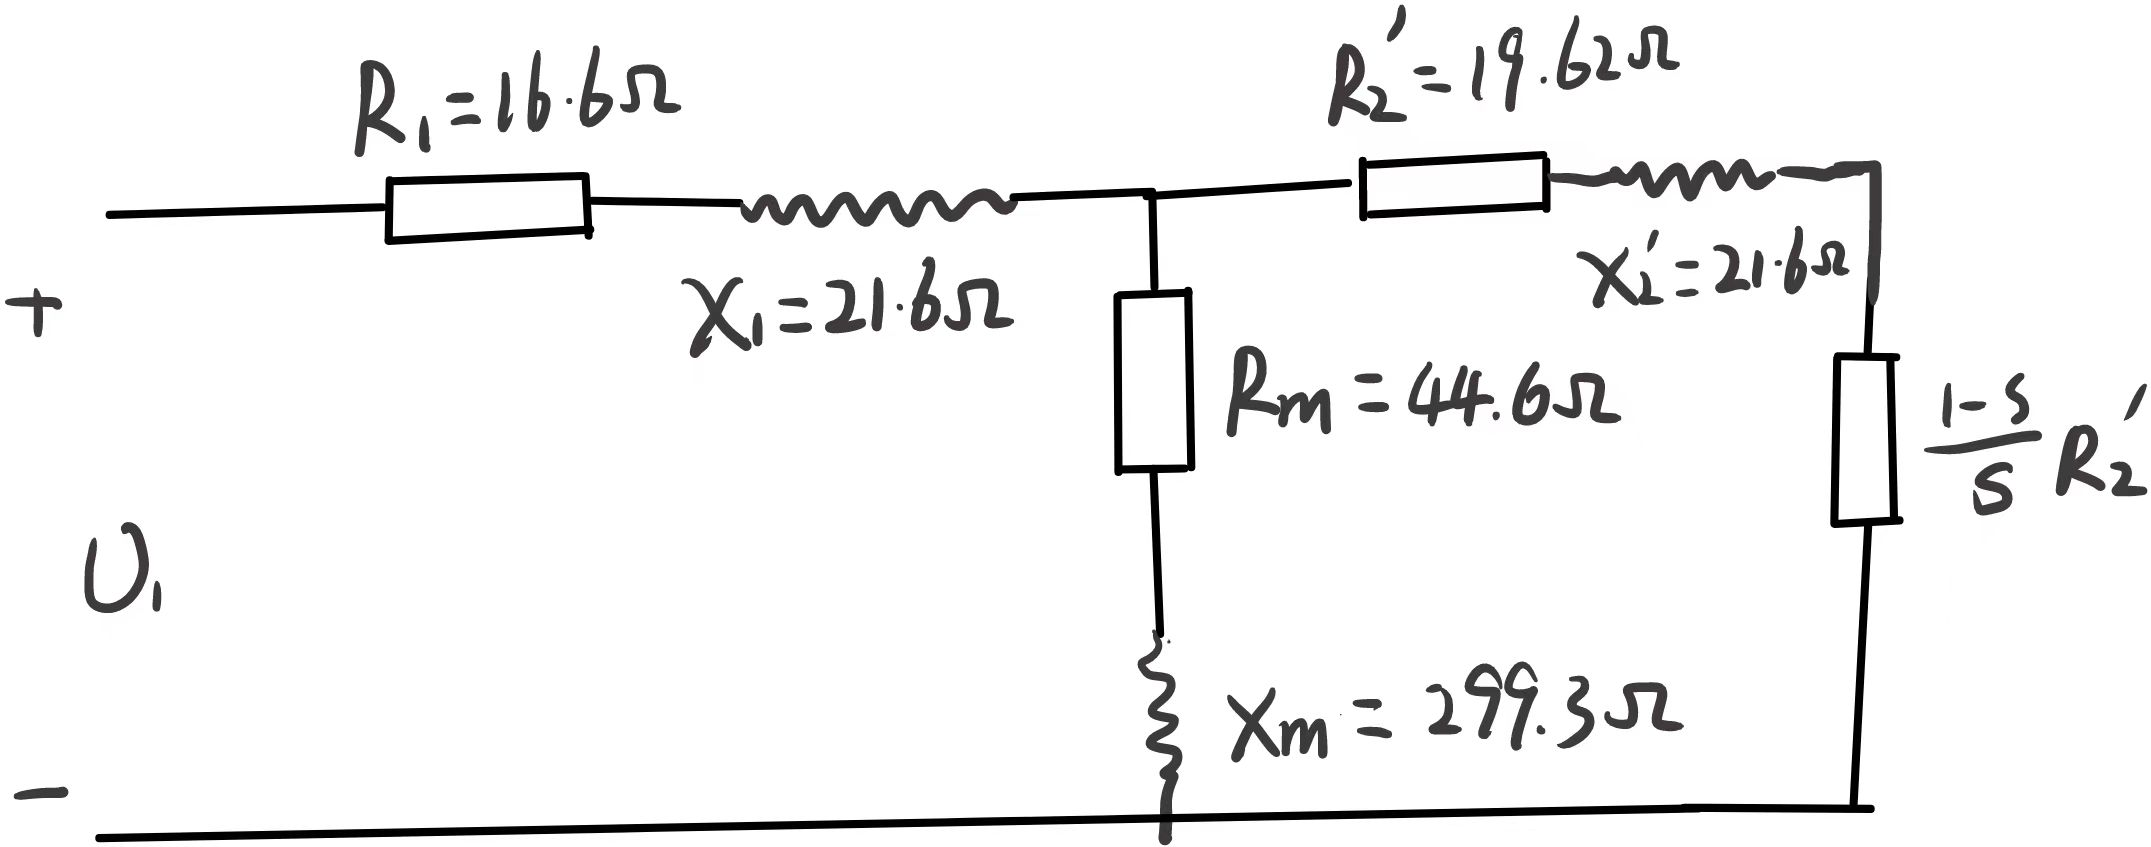
\includegraphics[width=0.8\textwidth]{./images/6.jpg}
\end{figure}


\subsection{负载实验}

\subsubsection{负载实验数据分析}

\begin{table}[H]
\centering
\small
\begin{tabular}{lrrrrrrr}
\toprule
$U_n$(V) & 220 & 220 & 220 & 220 & 220 & 220 & 220 \\
$I_a$ (A) & 0.673 & 0.585 & 0.505 & 0.462 & 0.44 & 0.39 & 0.378 \\
$I_b$ (A) & 0.666 & 0.575 & 0.5 & 0.467 & 0.441 & 0.4 & 0.393 \\
$I_c$ (A) & 0.636 & 0.533 & 0.466 & 0.437 & 0.418 & 0.372 & 0.367 \\
$P_{\text{I}}$ (W) & 54.69 & 39.96 & 21.65 & 12.06 & 4.57 & -12.5 & -22.1 \\
$P_{\text{II}}$ (W) & 136.1 & 113.1 & 95.22 & 85.91 & 78 & 60.6 & 50.61 \\
$T_2$ (N·m) & 1.04 & 0.82 & 0.61 & 0.5 & 0.41 & 0.2 & 0 \\
$n$(rpm) & 1370 & 1395 & 1420 & 1431 & 1440 & 1463 & 1478 \\
\midrule
$I$ (A) & 0.658 & 0.564 & 0.490 & 0.455 & 0.433 & 0.387 & 0.379 \\
$P_1$ (W) & 190.79 & 153.06 & 116.87 & 97.97 & 82.57 & 48.1 & 28.51 \\
$P_2$ (W) & 149.20 & 119.79 & 90.71 & 74.93 & 61.83 & 30.64 & 0 \\
$\eta$ & 0.782 & 0.783 & 0.776 & 0.765 & 0.749 & 0.637 & 0 \\
$\cos\varphi$ & 0.761 & 0.712 & 0.626 & 0.565 & 0.500 & 0.326 & 0.197 \\
\bottomrule
\end{tabular}
\end{table}

\subsubsection{实验工况与数据说明}

负载实验在额定电压$U_N = 220$ V条件下进行，通过逐步改变负载转矩，测量三相电机在不同负载工况下的电流、输入功率、转速以及输出转矩等参数。实验采用两瓦特计法测量三相输入功率，并由测功装置获得负载转矩。

\subsubsection{转速-负载转矩特性分析(机械特性)}
\begin{figure}[H]
    \centering
    \caption{转速-负载转矩特性}
    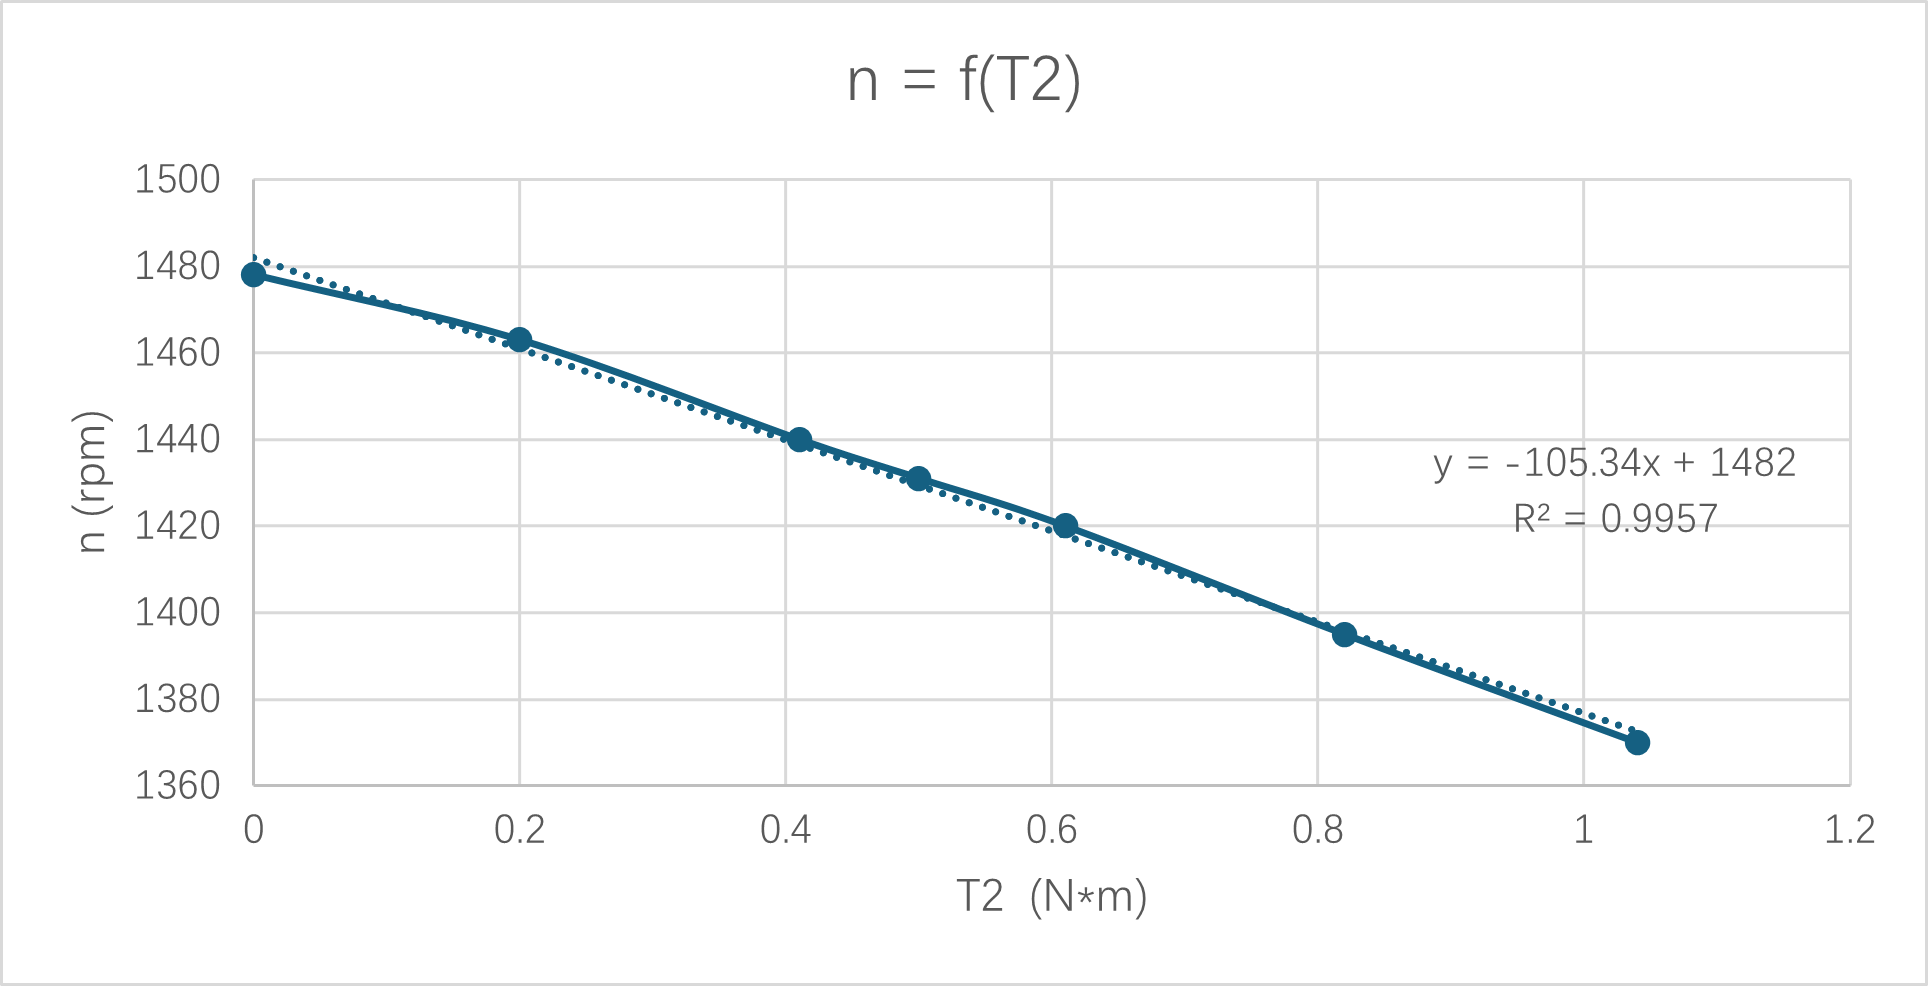
\includegraphics[width=1\textwidth]{./images/图片5.png}
\end{figure}
数据变化规律：
\begin{itemize}
\item 空载时转速约1478 r/min
\item 额定附近负载时转速降至1370 r/min
\item 转速变化范围约7\%
\end{itemize}

由实验数据可知，随着负载转矩的增大，电机转速逐渐下降，呈线性变化，但整体变化幅度较小，表明三相异步电机具有较"硬"的机械特性。这是异步电机的典型运行特征，即通过转差率的变化来适应负载变化。实验结果与异步电机机械特性理论分析一致。

\subsubsection{输出功率-负载特性分析}
\begin{figure}[H]
    \centering
    \caption{输出功率-负载转矩特性}
    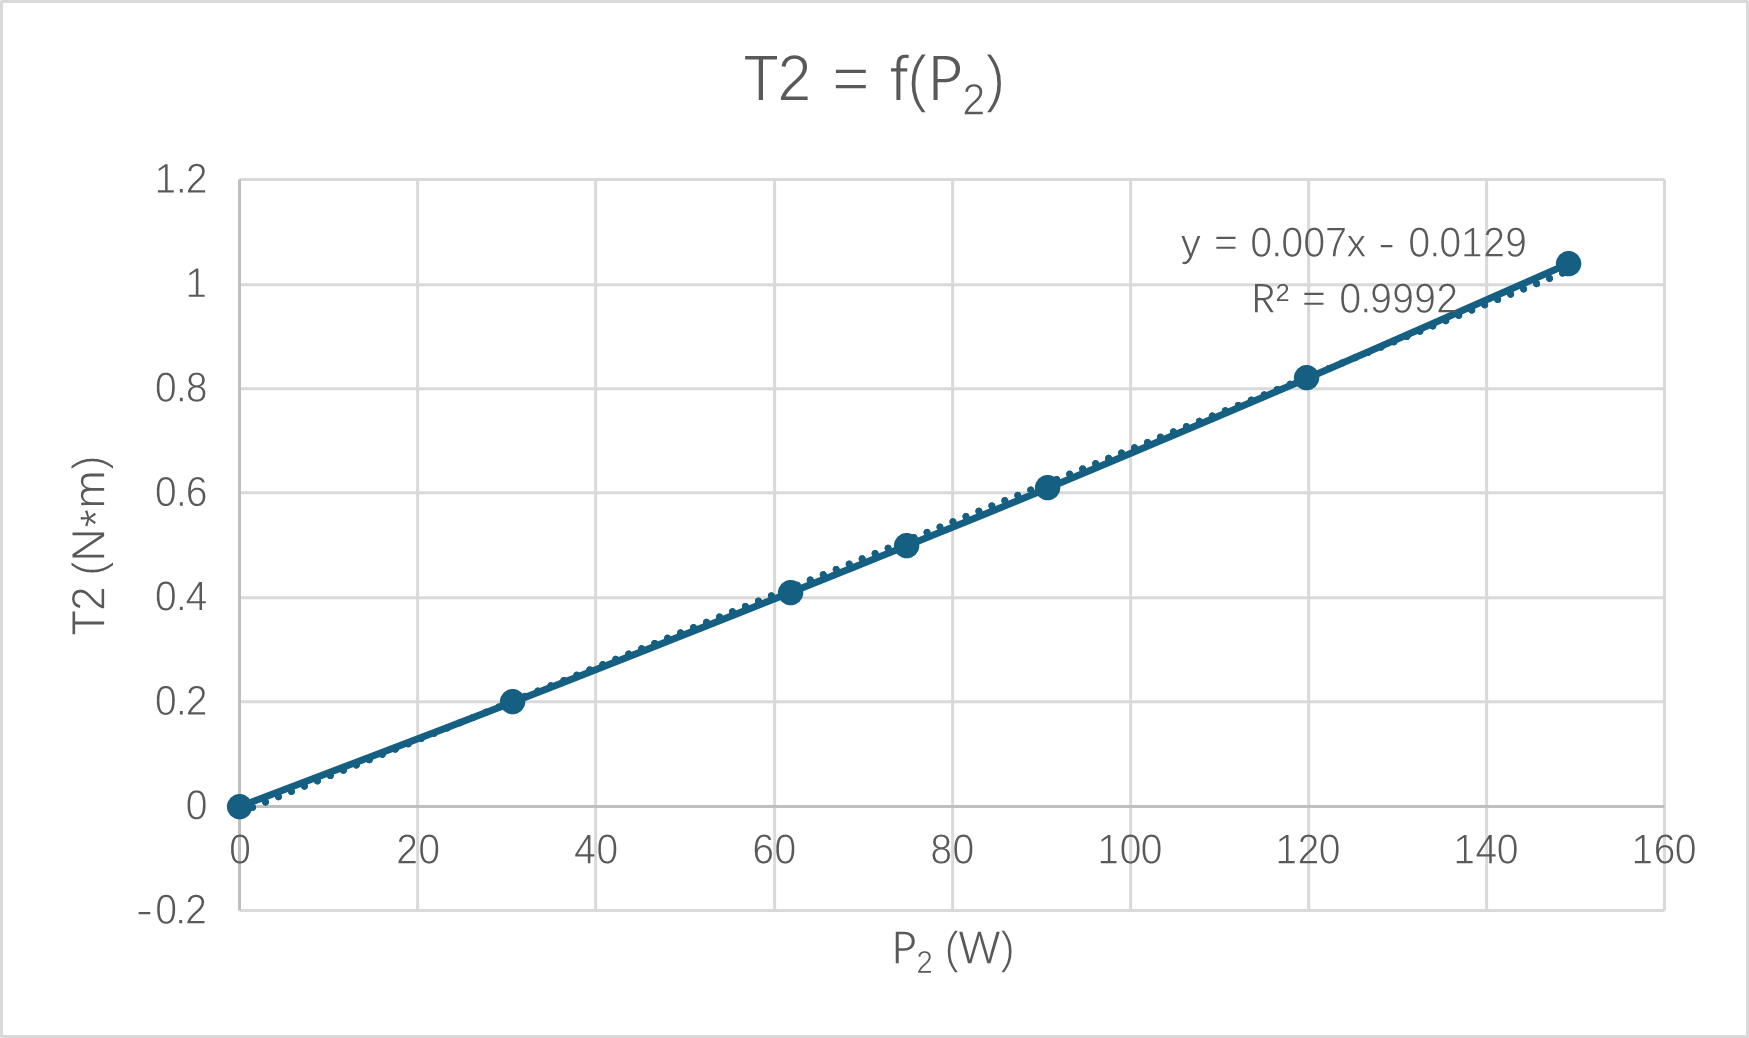
\includegraphics[width=0.8\textwidth]{./images/图片9.png}
\end{figure}
输出功率计算公式：
\begin{equation*}
P_2 = \frac{2\pi n}{60}T_2
\end{equation*}

在负载实验中，电机在额定电压下运行，转速随负载变化幅度较小，因此输出功率主要受负载转矩变化的影响。因此输出功率与负载成正相关，输出功率随负载增大而增大。
因而可以用输出功率来等效负载转矩。
\subsubsection{三相电流与负载变化关系分析}
\begin{figure}[H]
    \centering
    \caption{电流-负载转矩特性}
    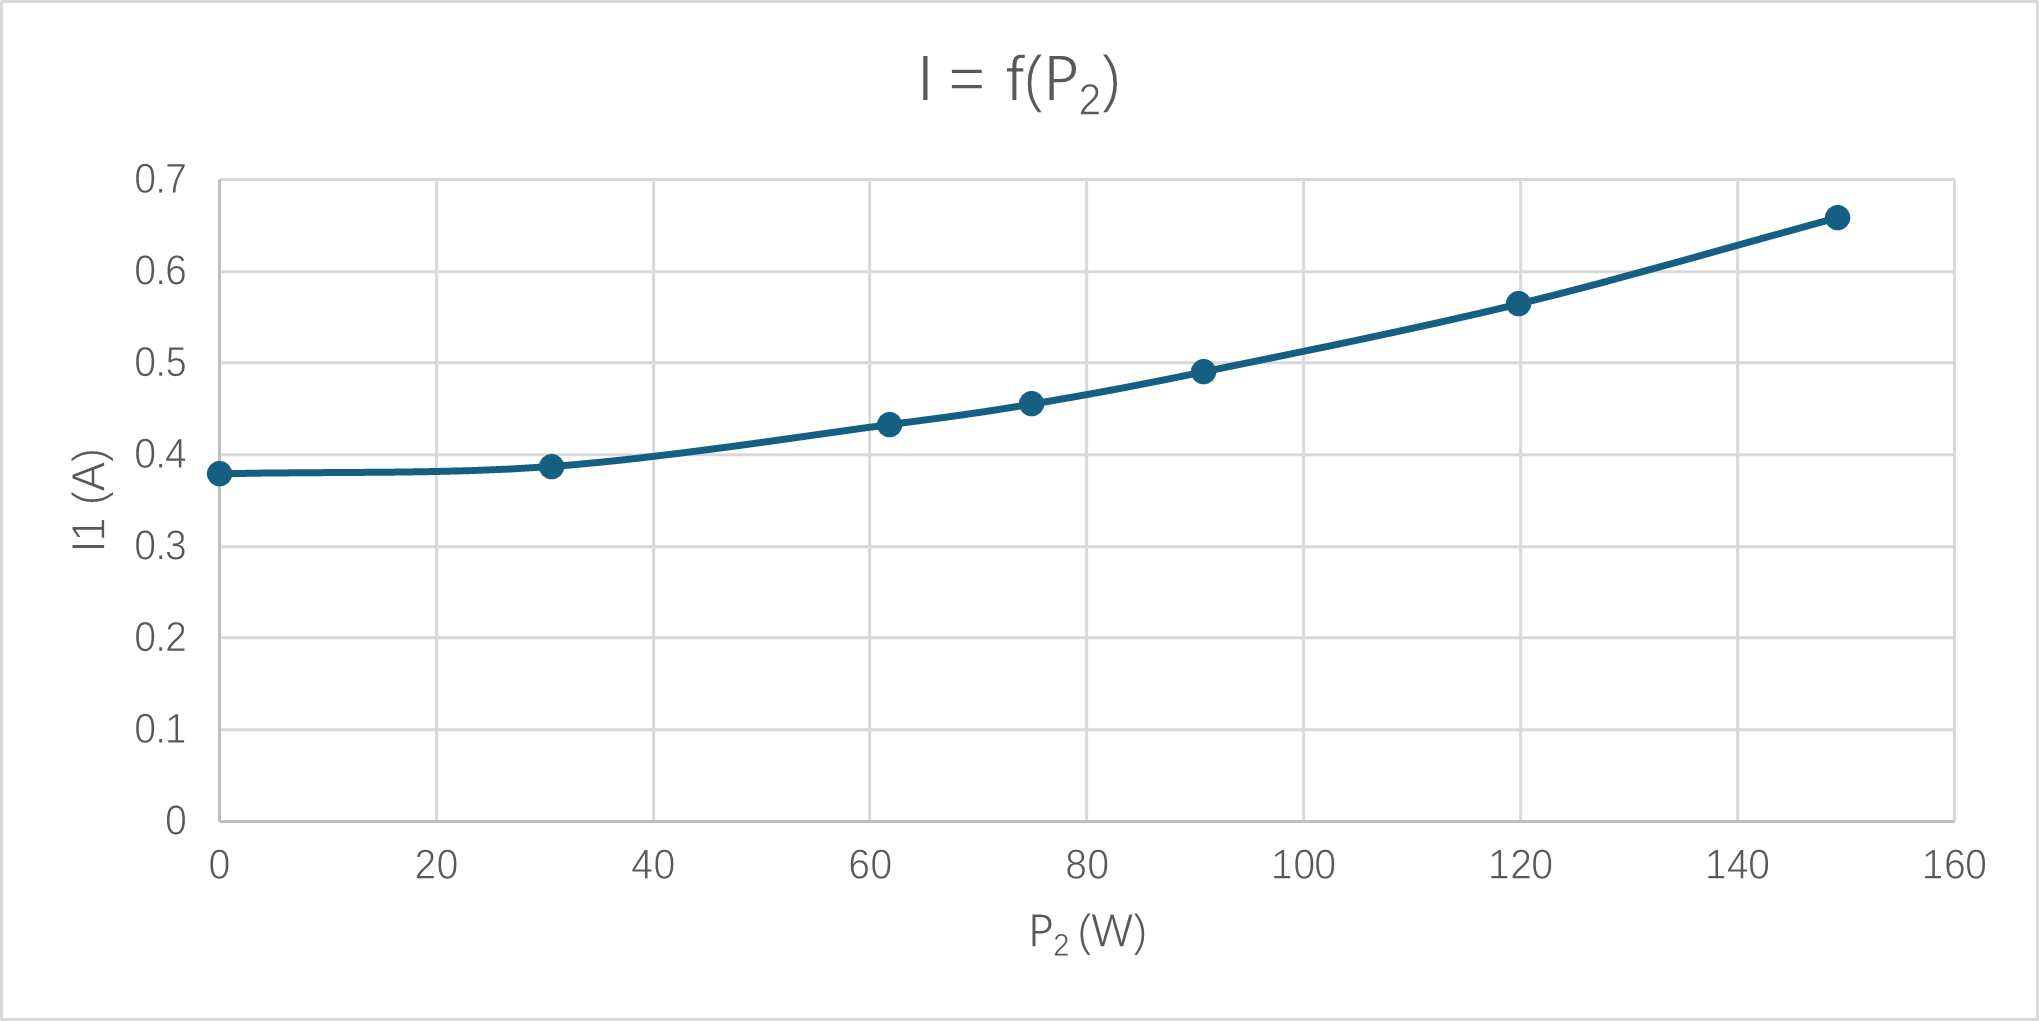
\includegraphics[width=1\textwidth]{./images/图片7.png}
\end{figure}
根据实验数据计算得到三相平均电流：
\begin{equation*}
I = \frac{I_a + I_b + I_c}{3}
\end{equation*}

数据特征与分析：随着负载转矩由0增加至1.04 N·m，电流由0.38 A增加至0.66 A，三相电流幅值接近，最大偏差较小。

从实验结果可以看出，电机在额定电压下运行时，定子电流随负载转矩的增加而明显增大。这是由于负载加重使电机转差率增大，转子电流及定子感应电流相应增加，从而导致定子电流上升。当负载很小的时候电流主要是励磁电流和空载电流，因此图像趋于一个定值。同时，各工况下三相电流数值接近，表明电机三相绕组及电源具有较好的对称性，实验数据具有较高的可信度。

\subsubsection{输入功率与负载特性分析}
\begin{figure}[H]
    \centering
    \caption{输入功率-输出功率转矩特性}
    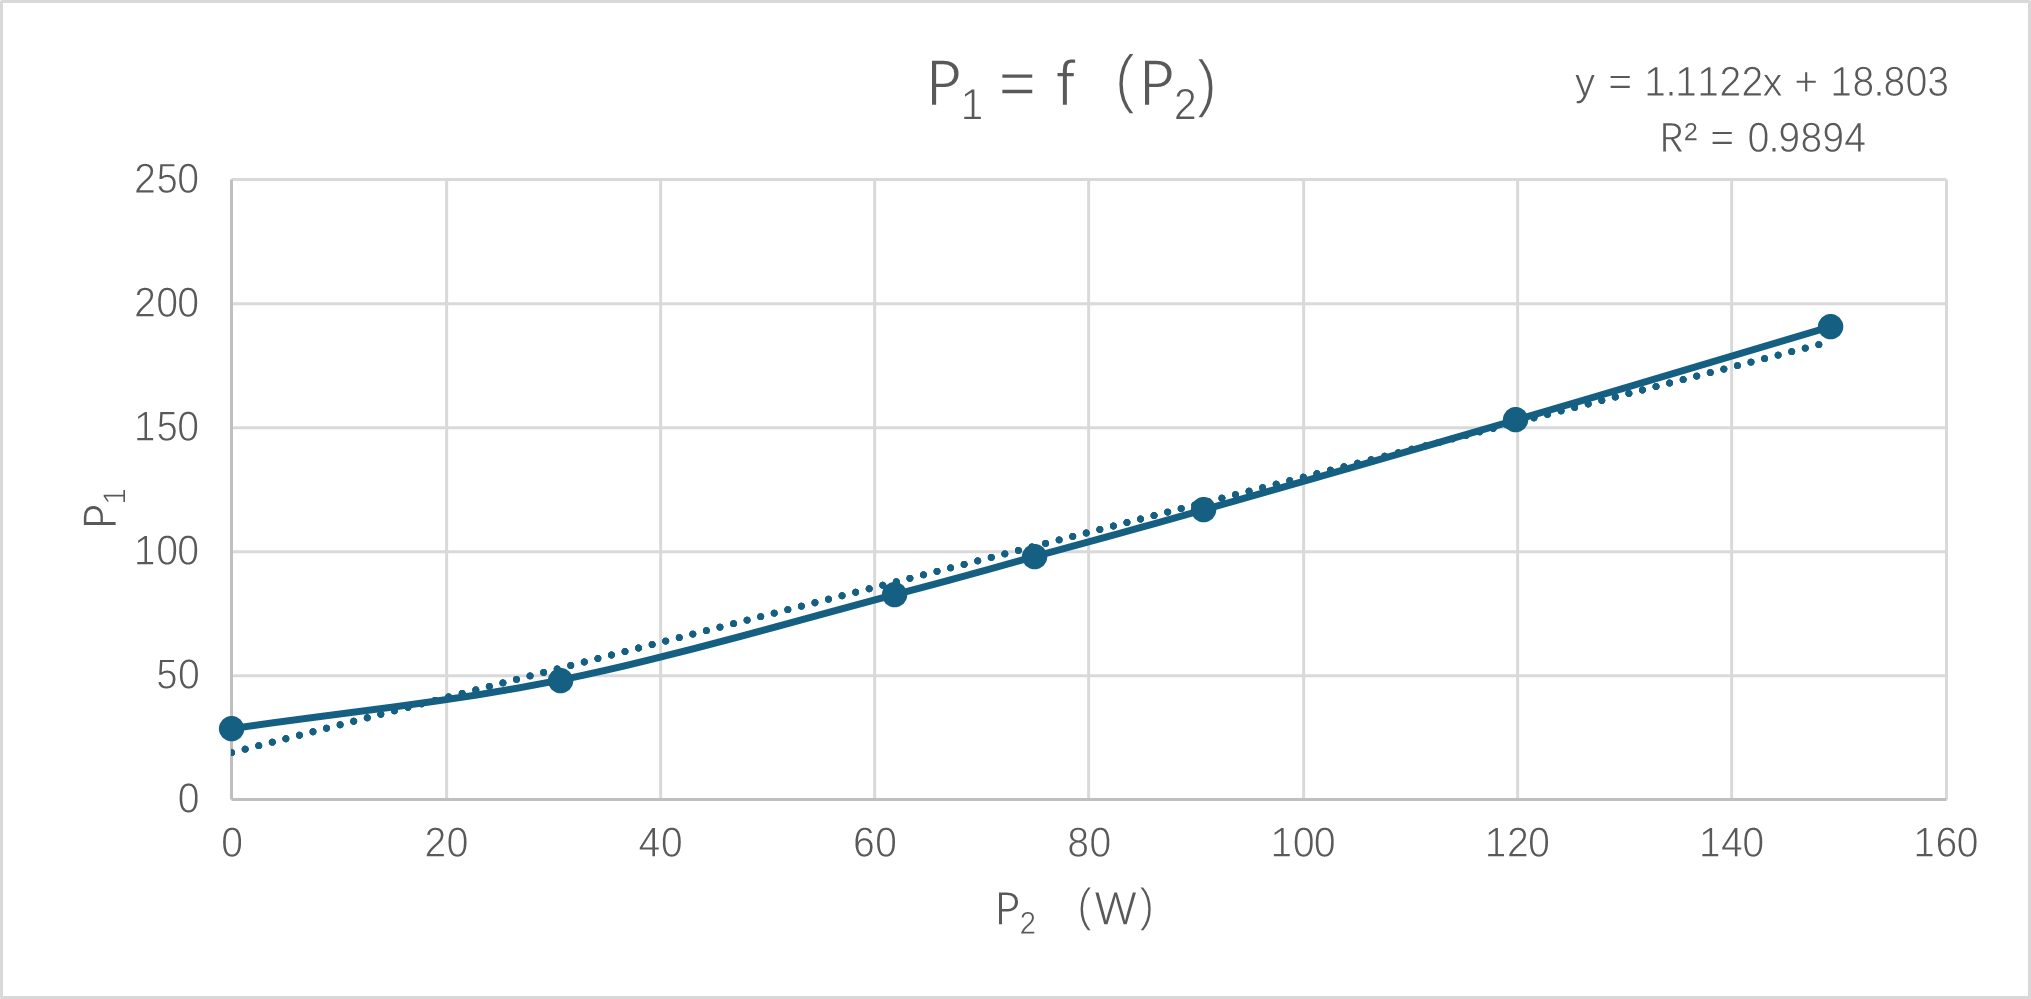
\includegraphics[width=1\textwidth]{./images/图片15.png}
\end{figure}
三相输入功率采用两瓦特计法计算：
\begin{equation*}
P = |P_1 + P_2|
\end{equation*}

当负载很小时，输出功率趋于0，输入功率主要是拿来产生铁损耗和铜损耗与空载损耗所以输入功率不为0。负载增大时，输入功率由28.5 W增至190.8 W，随着负载转矩的增大，电机输入功率显著增加。这是由于负载加重后，电机输出机械功率及铜损均明显增大。

\subsubsection{功率因数随负载变化的分析}
\begin{figure}[H]
    \centering
    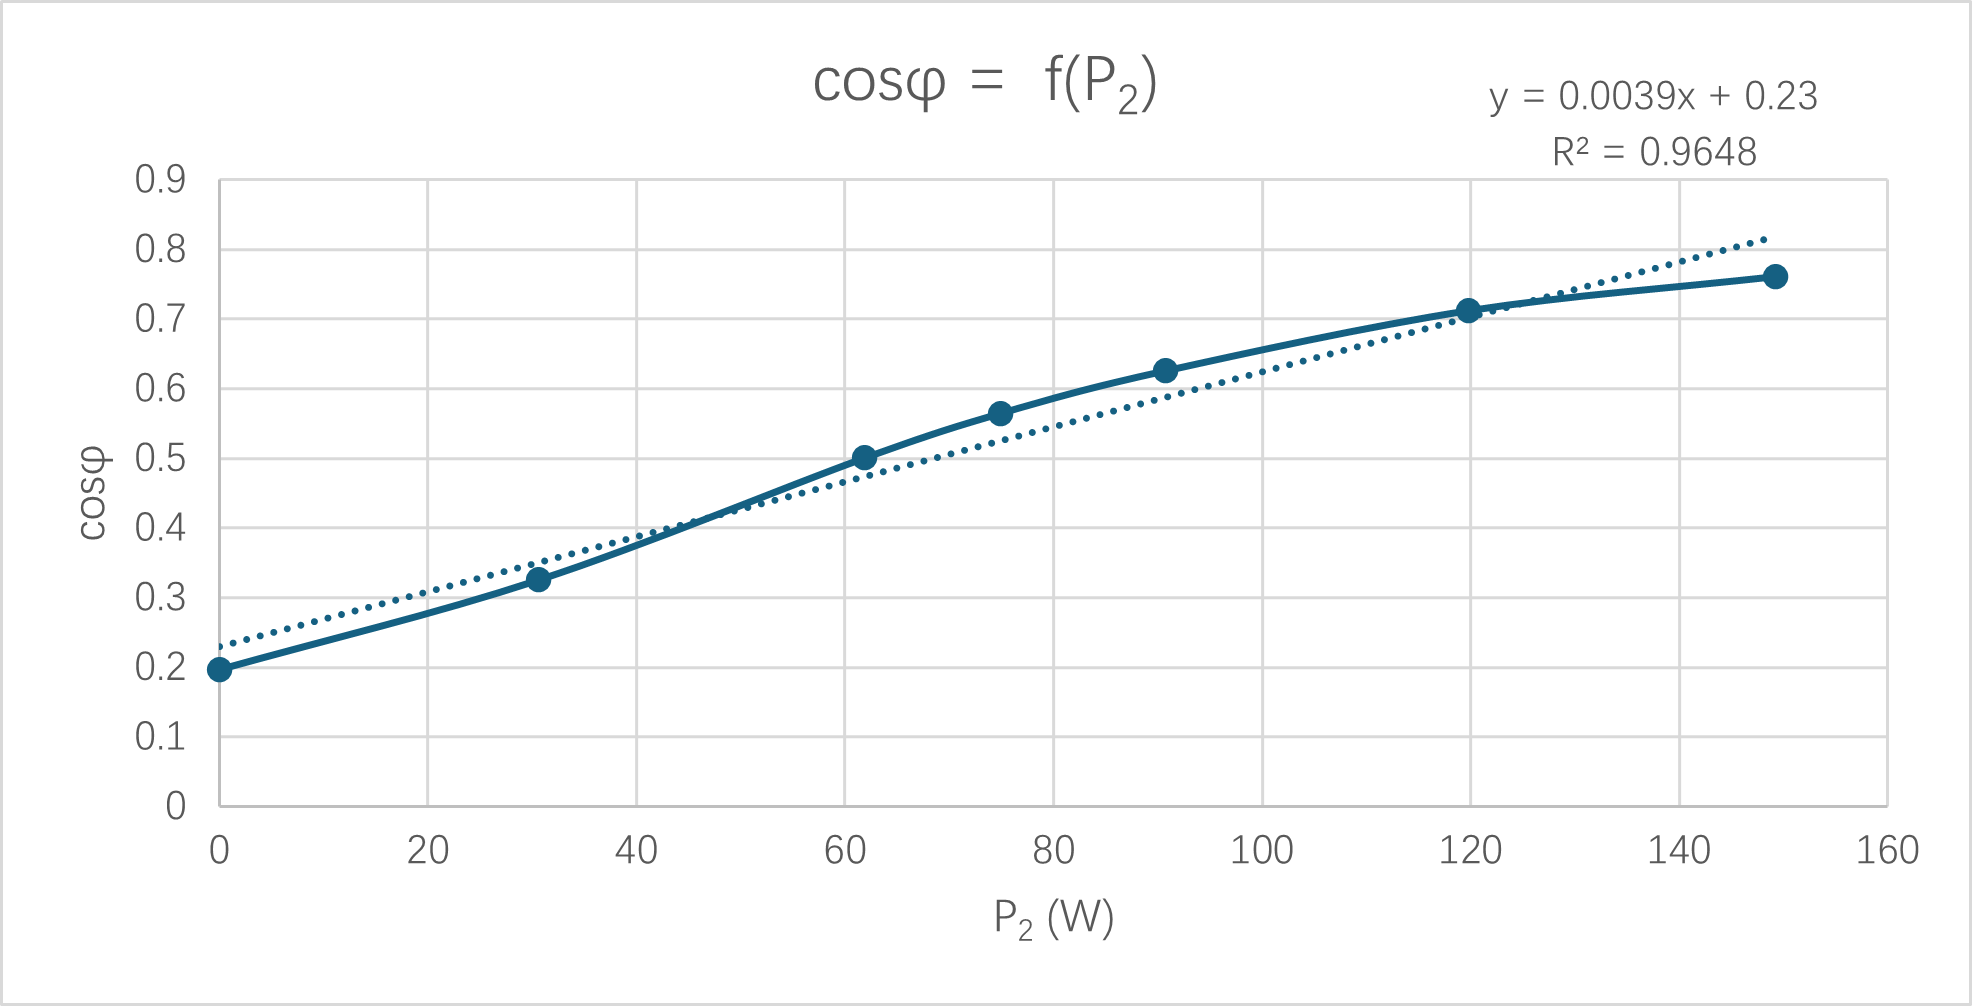
\includegraphics[width=1\textwidth]{./images/图片12.png}
\end{figure}
根据实验数据计算功率因数：
\begin{equation*}
\cos\varphi = \frac{P}{\sqrt{3}UI}
\end{equation*}

实验结果表明，电机功率因数随负载的增加而明显提高。在轻载及空载条件下，电机主要消耗励磁电流，功率因数较低；随着负载加重，有功电流分量增加，使得功率因数逐渐提高。该变化趋势符合异步电机运行特性。

\subsubsection{效率-负载特性分析}
\begin{figure}[H]
    \centering
    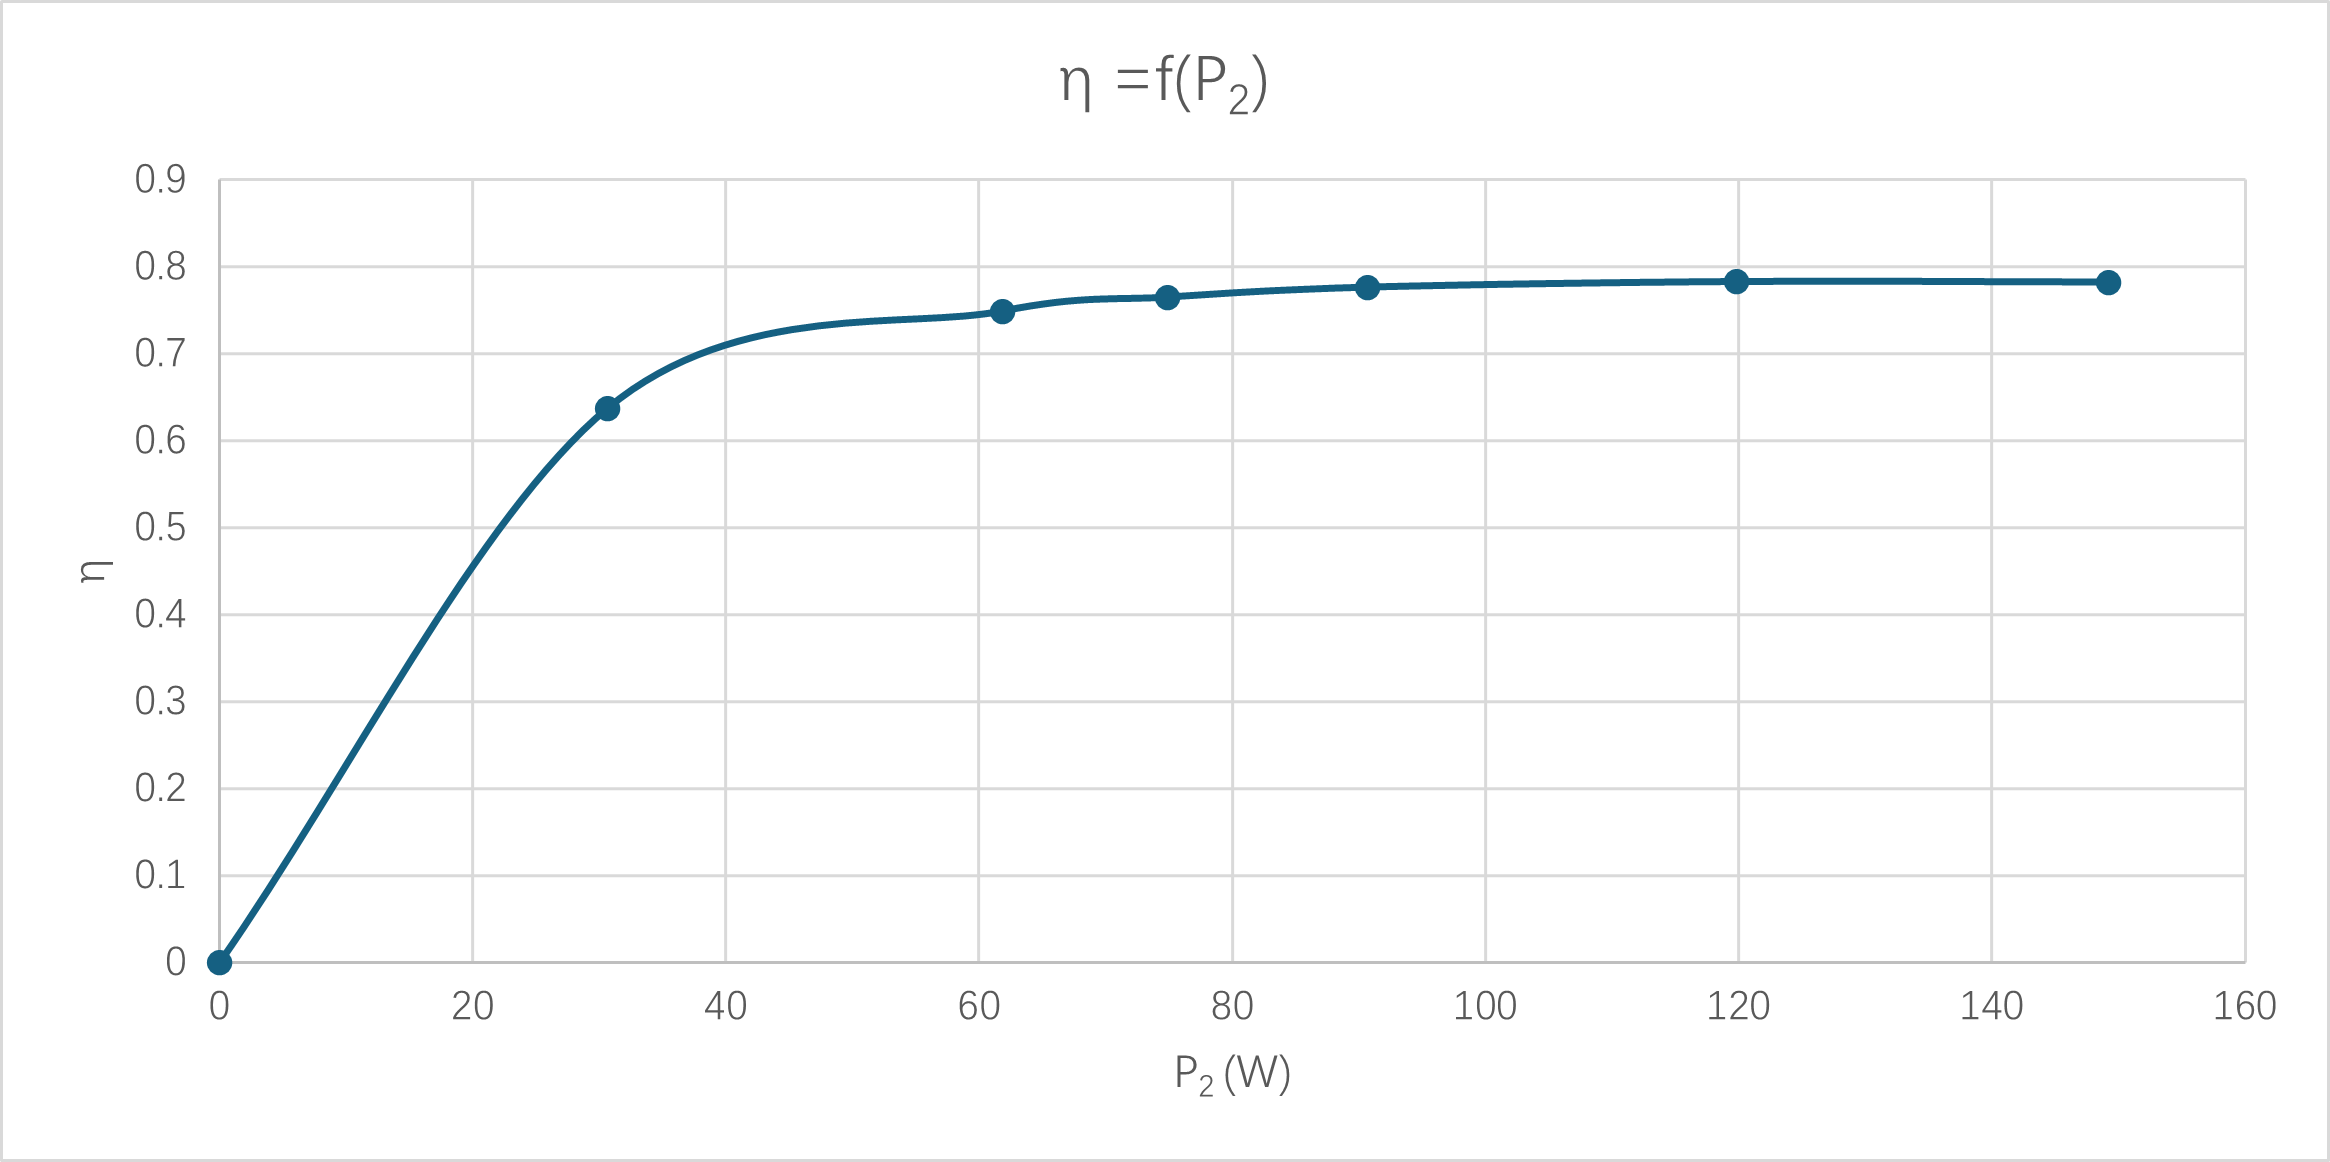
\includegraphics[width=1\textwidth]{./images/图片11.png}
\end{figure}
效率计算公式为：
\begin{equation*}
\eta = \frac{P_{\text{out}}}{P_{\text{in}}} = \frac{P_2}{P_1}
\end{equation*}

实验数据呈现的规律：
\begin{itemize}
\item 效率在中等负载附近达到最大值(约78\%)
\item 轻载与空载时效率明显偏低
\end{itemize}

从实验结果可以看出，电机效率随负载增加呈现"先升高后趋于平缓"的变化趋势，并在中等负载附近达到最大值。这是由于在轻载条件下，铁损和机械损耗在总损耗中占比较大；随着负载增加，有效输出功率占比提高，使效率上升。

当负载继续增大时，铜损迅速增加，抵消了输出功率增加带来的效率提升，使效率增长趋于平缓。
\subsection{星角启动实验数据分析}
\subsubsection{星角启动实验数据}
\noindent Y 形时电流 $I_Y =$ \underline{ 0.215\hspace{3cm}} A\\
$\Delta$ 形时电流 $I_\Delta = $ \underline{  0.63\hspace{3cm}} A
\subsubsection{电流比}
\noindent 理论值：IΔ/IY = 3.0\\
实测值：0.63/0.215 ≈ 2.93\\
误差 < 3 \%，与理论几乎完全吻合
\subsubsection{与全压直接启动对比}
若直接 Y 接、220 V 起动，起动电流0.63A
星-角启动把起动电流从 0.63 A 降到 0.215 A，降低约 3 倍，把起动电压从 220V 下降到 127V
，降低约$\sqrt{3}$倍，启动转矩正比于U的平方，实现起动转矩下降3倍，满足“降压→降流→降启动转矩”目标。
与理论相符合。
\subsection{调速实验数据处理与分析}

\subsubsection{调速实验数据}

\begin{table}[H]
\centering
\caption{调定子电压调速实验($R_r=0$Ω)}
\begin{tabular}{lrrrrrrrr}
\toprule
\multicolumn{8}{c}{$T=0$} \\
\midrule
$U$ & 220 & 197.7 & 176 & 153.9 & 131.3 & 110.6 & 88.33 \\
$n$ & 1479 & 1471 & 1467 & 1456 & 1447 & 1429 & 1398 \\
\midrule
\multicolumn{8}{c}{$T=0.2$} \\
\midrule
$U$ & 219.3 & 197.1 & 176 & 154 & 131.7 & 109.5 & 88.5 \\
$n$ & 1464 & 1453 & 1449 & 1437 & 1414 & 1374 & 1287 \\
\bottomrule
\end{tabular}
\end{table}

\begin{table}[H]
\centering
\caption{调转子电阻调速实验($U_n=220$ V)}
\begin{tabular}{lrrrrr}
\toprule
\multicolumn{6}{c}{$T=0$} \\
\midrule
$R_r$ & 0 & 2 & 5 & 15 & $\infty$ \\
$n$ & 1477&	1472&	1463&	1445&	1433 \\
\midrule
\multicolumn{6}{c}{$T=0.2$} \\
\midrule
$R_r$ & 0 & 2 & 5 & 15 & $\infty$ \\
$n$ & 1466 & 1459 & 1453 & 1437 & 1382 \\
\bottomrule
\end{tabular}
\end{table}

\subsubsection{调速实验说明}

调速实验在异步电机运行过程中，通过改变定子电压或改变转子回路电阻，研究电机转速随控制参数变化的规律。实验分别在空载($T = 0$)和轻载($T = 0.2$ N·m)两种工况下进行，以对比负载对调速特性的影响。

\subsubsection{调定子电压调速特性分析}
\begin{figure}[H]
    \centering
    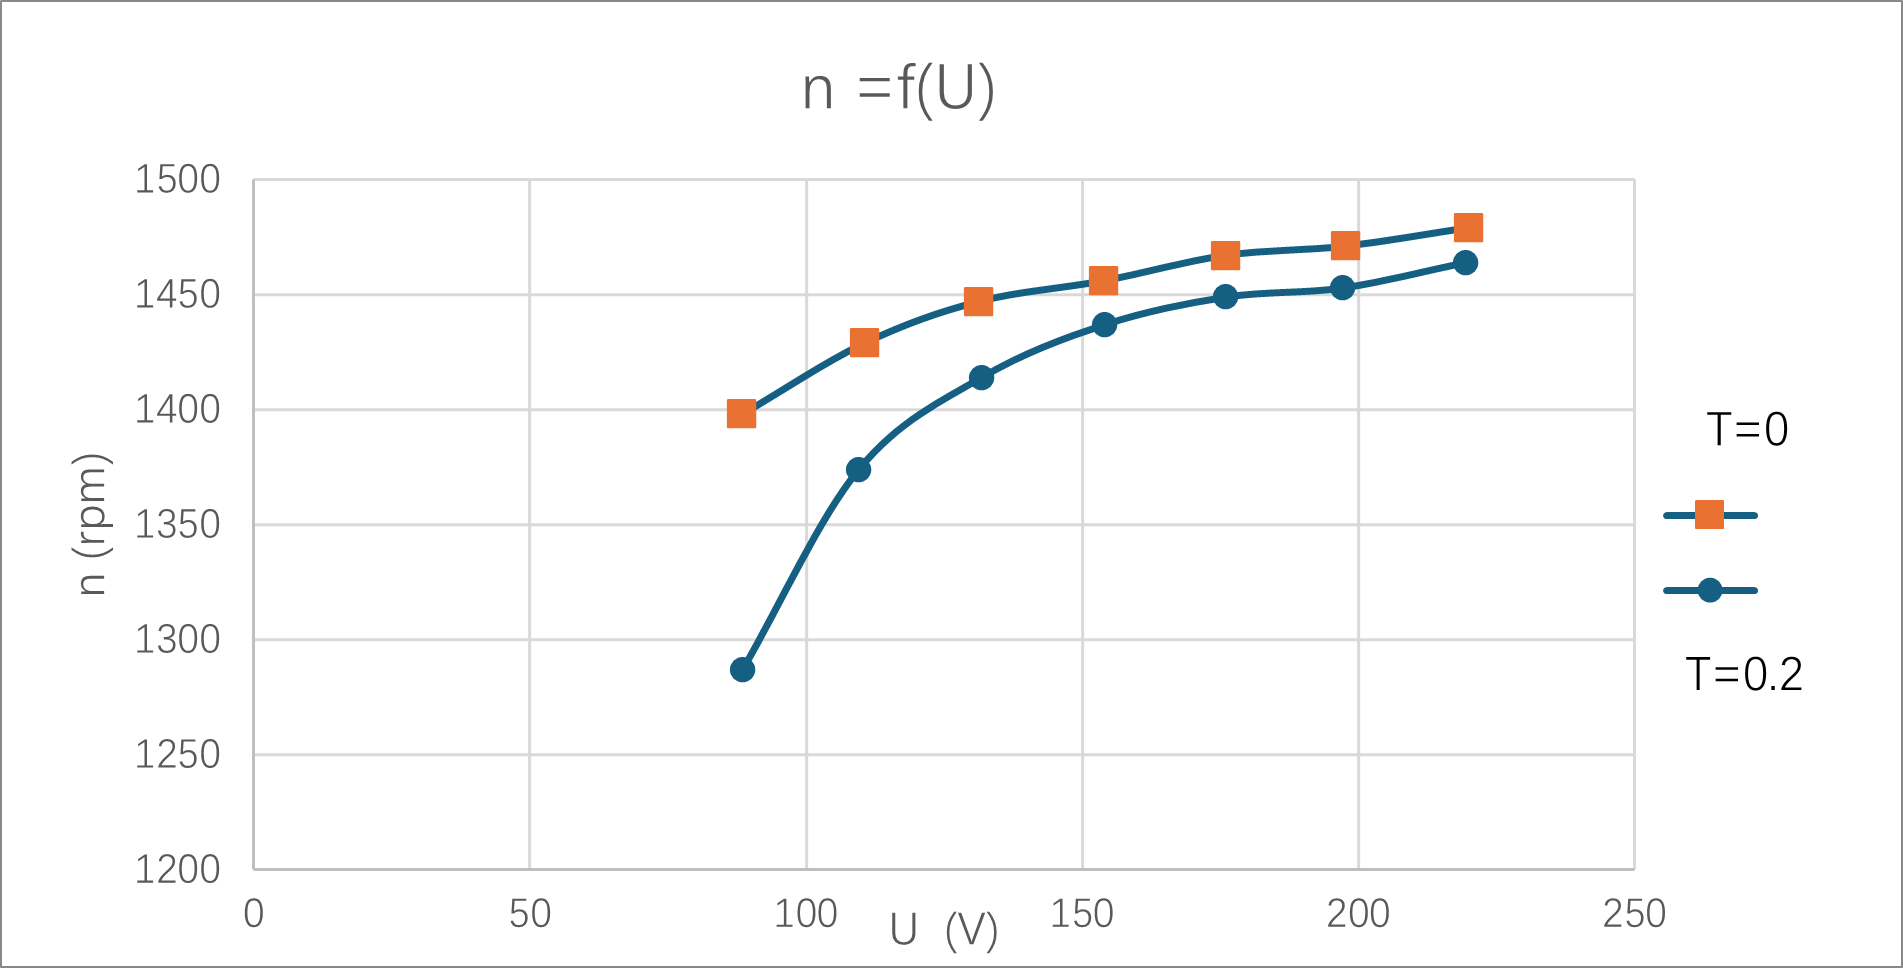
\includegraphics[width=1\textwidth]{./images/图片13.png}
\end{figure}
\textbf{(1) 空载工况$T = 0$}

在空载条件下，改变定子电压$U$，测得转速$n$的变化情况如下：
\begin{itemize}
\item 电压由220 V降至88.33 V
\item 转速由1479 r/min降至1398 r/min
\item 转速变化幅度较小(约5.5\%)
\end{itemize}

在空载条件下，随着定子电压的降低，电机转速呈缓慢下降趋势，但整体变化幅度较小。这是由于空载时电机转差率极小，转速主要由同步转速决定，电压变化对转速影响有限。因此，调压方式在空载条件下的调速效果不明显。

\textbf{(2) 轻载工况$T = 0.2$ N·m}

在轻载条件下：
\begin{itemize}
\item 电压由219.3 V降至88.5 V
\item 转速由1464 r/min降至1287 r/min
\end{itemize}

在轻载条件下，随着定子电压降低，电机转速下降幅度明显增大。这是由于在负载作用下，降低定子电压会使电磁转矩减小，为维持负载转矩，电机必须通过增大转差率来平衡，从而导致转速显著下降。

因此，与空载相比，调压调速在负载条件下对转速的影响更为明显。

\subsubsection{调转子电阻调速特性分析($U_n = 220$ V)}
\begin{figure}[H]
    \centering
    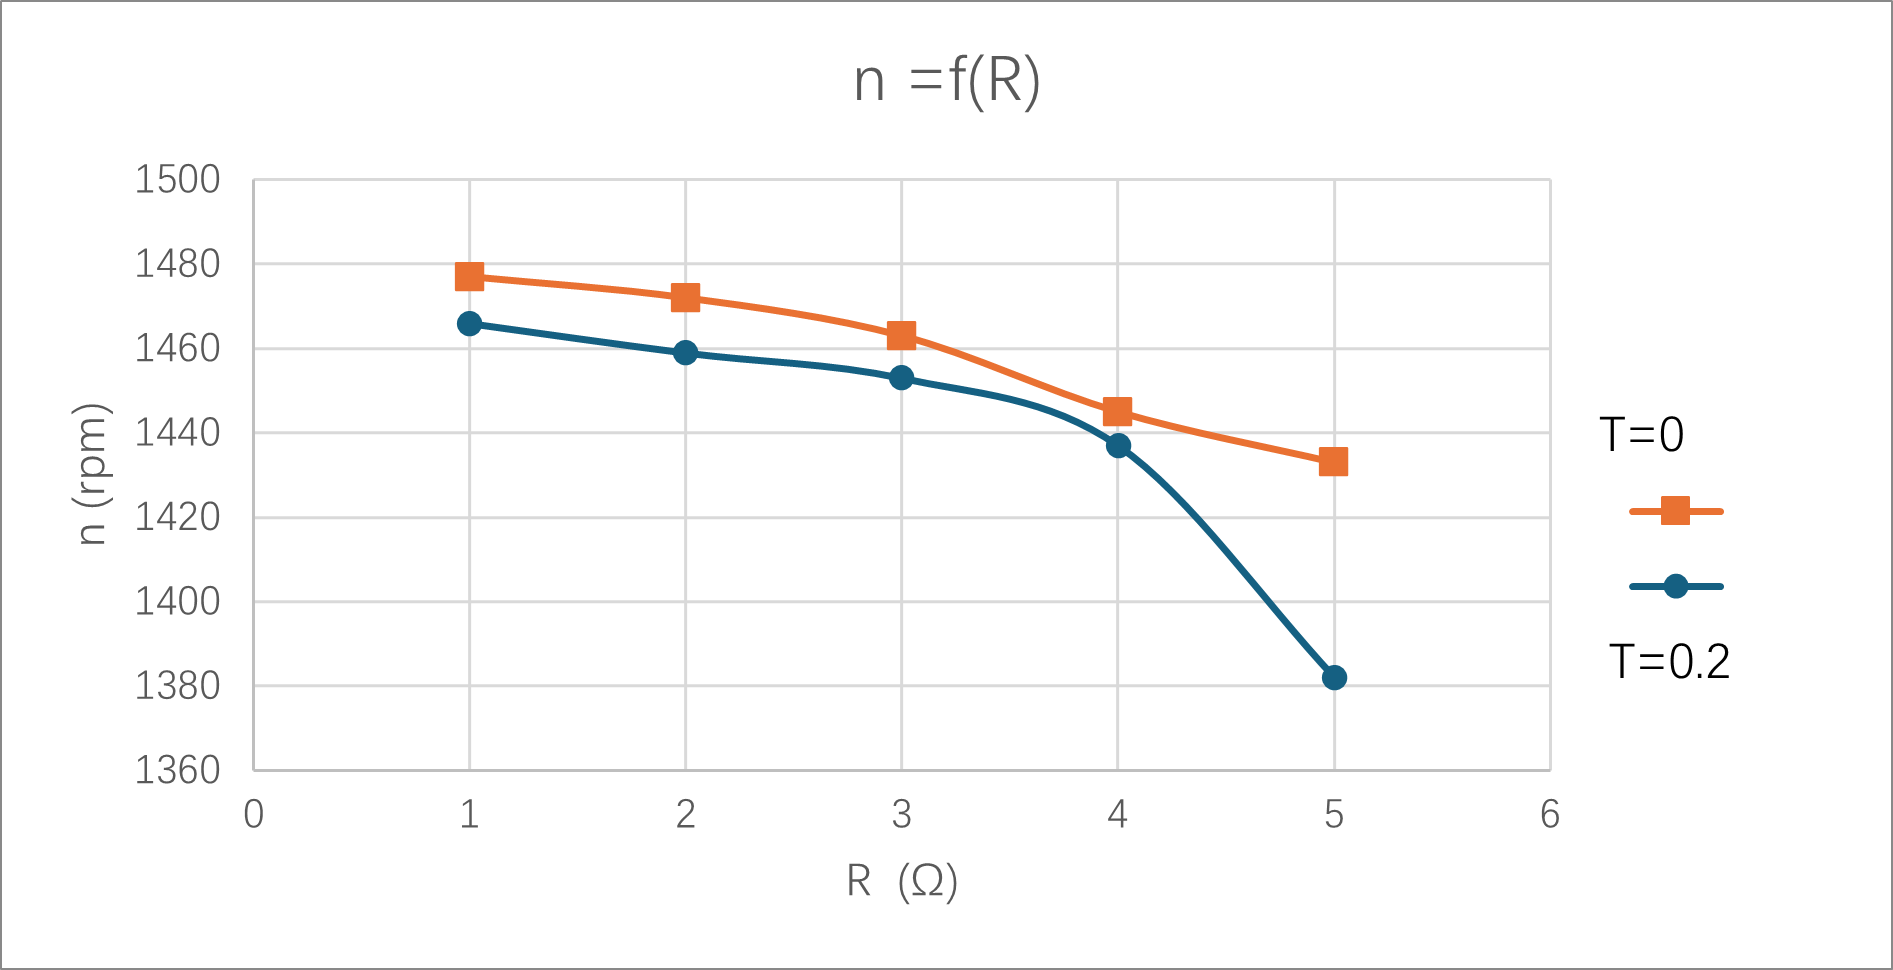
\includegraphics[width=1\textwidth]{./images/图片14.png}
\end{figure}
调转子电阻实验在定子电压保持额定值条件下进行，通过改变转子回路外接电阻$R_r$，测量转速变化。

\textbf{(1) 空载工况$T = 0$}
\begin{itemize}
\item 外接电阻由0增加至$\infty$
\item 转速由1477 r/min降至1433 r/min
\item 转速变化不大
\end{itemize}

在空载条件下，随着转子回路外接电阻的增大，电机转速略有下降，但变化幅度较小。这是由于空载时电磁转矩需求较低，转差率始终保持较小值，因此转子电阻变化对转速影响有限。

\textbf{(2) 轻载工况$T = 0.2$ N·m}
\begin{itemize}
\item 转子电阻增大时，转速由1466 r/min降至1382 r/min
\item 转速下降幅度明显大于空载工况
\end{itemize}

在轻载条件下，随着转子回路电阻的增大，电机转速明显下降。这是由于转子电阻增大会使电磁转矩特性曲线向低速方向移动，为维持负载转矩，电机需在较大的转差率下运行，从而导致转速降低。

调转子电阻方式在负载条件下具有较明显的调速效果。

\subsubsection{调速实验结论}

调定子电压调速方式结构简单，但调速范围有限，且负载能力随电压降低而显著下降，仅适用于风机、水泵等对转速精度要求不高的场合。

调转子电阻调速具有起动转矩大、调速平滑等优点，但其缺点是转子铜损显著增加，效率较低，通常仅适用于绕线式异步电机的起动及短时调速场合。

\section{总结与体会}
本次三相异步电机综合实验围绕空载、短路、负载及调速四条特性展开，
系统测取了电机在 0～1.05 N·m 范围内的运行数据，
并基于 T 型等效电路模型，得到了电机的参数。
通过这次试验，我学会了如何使用两瓦特计法测量三相功率，
掌握了异步电机的基本运行特性，并理解了等效电路参数的物理意义。
此外，实验过程中还锻炼了数据处理与分析能力，
为今后深入学习类似的学习与实验打下了坚实基础。
\end{document}
